%%%%%%%%%%%%%%%%%%%%%%%%%%%%%%%%%%%%%%%%%%%%%%%%%%%%%%%%%%%%%%%%%
%                                                               % 
%%%%%%%%%%%%%%%%%%%%%%%%%%%%%%%%%%%%%%%%%%%%%%%%%%%%%%%%%%%%%%%%%
\documentclass{dmathesis}
%% uncommand the following line to print equation labels next to
%% equation numbers. 
% \usepackage{showlabel}
\usepackage{xcolor}
\usepackage{graphicx}
\usepackage{array}
\usepackage{amsmath}
\usepackage{listings} % Required for code listing
% \usepackage{color,soul}
% \usepackage[dvipsnames]{xcolor}

% Define code listing settings
\lstset{
    language=Python, % Set language
    basicstyle=\ttfamily\small, % Set font style and size
    breaklines=true, % Enable automatic line breaking
    keywordstyle=\color{blue}, % Set keyword color
    stringstyle=\color{red}, % Set string color
    commentstyle=\color{green!60!black}, % Set comment color
    numbers=left, % Line numbers on left
    numberstyle=\tiny\color{gray}, % Line number style
    % backgroundcolor=\color{lightgray!20}, % Background color
    captionpos=b, % Caption position: bottom
    tabsize=4, % Tab size
    showspaces=false, % Don't show spaces
    showstringspaces=false, % Don't show spaces in strings
}

%% The following is to control the format of your thesis
\input{format}

%% File to be included while running latex.
\includeonly{1_Intro, 2_Lit_Rev, 3_Prop_Meth, 4_Res_Dis, 5_Conclusion, 6_Project_Outreach, 7_Ref, 8_Vision_Mission}

\begin{document}
%% Front page of thesis
\pagenumbering{roman}
%\pagenumbering{arabic}

\setcounter{page}{1}

\fancypagestyle{plain}{%
\fancyfoot[R]{}
\renewcommand{\headrulewidth}{0.4pt}
}

\newpage
\thispagestyle{empty}
\begin{center}
  {\large \bf PROJECT PHASE 1 REPORT}\\
ON\\
  {\huge \bf Real-Time Segmentation and}\\
   \vspace{0.5 cm}
   {\huge \bf Labelling of Objects in Videos}\\
   \large Submitted by\\
   { \bf Ajay T Shaju (SJC20AD004)}\\
   { \bf Emil Saj Abraham (SJC20AD028)}\\
   { \bf Justin Thomas Jo (SJC20AD046)}\\
   { \bf Vishnuprasad K G (SJC20AD063)}\\[-0.6mm]
  {\large to\\[-0.6mm] the APJ Abdul Kalam Technological University\\[-0.6mm] in partial fulfillment of the requirements for the award of the degree\\[-0.6mm] of\\[-0.6mm] Bachelor of Technology\\[-0.6mm] in\\[-0.6mm] {\bf Artificial Intelligence and Data Science}}
  
  % Put your university logo here if you wish.
   \begin{center}
   \includegraphics[width=0.3\textwidth]{Images/SJCET_logo.png}
   \end{center}

  {\large {\bf Department of Artificial Intelligence and Data Science}\\
          [-3mm] {\bf St. Joseph's College of Engineering and Technology, Palai}\\
           [1mm]  December : 2023}

\end{center}
%%%%%%%%%%%%%%%%%%%%%%%%%%%%%%%%%%%%%%%%%%%%%%%%%%%%%%%%%%%%%%%%%%%%%%%%%%%
%%%%%%%%%%%%%%%%%%           The abstract page         %%%%%%%%%%%%%%%%%%%%  
%%%%%%%%%%%%%%%%%%%%%%%%%%%%%%%%%%%%%%%%%%%%%%%%%%%%%%%%%%%%%%%%%%%%%%%%%%%
\newpage
\thispagestyle{empty}
\addcontentsline{toc}{chapter}{\numberline{}Declaration}
\begin{center}
  \vspace*{1cm}
  \textbf{\large Declaration}
\end{center}
We undersigned hereby declare that the project phase 1 report on {\bf“Real-Time Segmentation And Labelling Of Objects In Videos”}, submitted for partial fulfillment of the requirements for the award of the degree of Bachelor of Technology of the APJ Abdul Kalam Technological University, Kerala, is a bonafide work done by us under the supervision of {\bf Dr. Deepa V}. This submission represents our ideas in our own words and where ideas or words of others have been included. We have adequately and accurately cited and referenced the original sources. We also declare that we have adhered to the ethics of academic honesty and integrity and have not misrepresented or fabricated any data, idea, fact, or source in our submission. We understand that any violation of the above will be a cause for disciplinary action by the institute and/or the University and can also evoke penal action from the sources which have thus not been properly cited or from whom proper permission has not been obtained. This report has not been previously formed the basis for the award of any degree, diploma, or similar title of any other University. 
\vspace{1.3 cm} \\
{{\bf Name and Signature of Students}\vspace{0.5 cm}\\
{ \bf Ajay T Shaju (SJC20AD004)}\\
{ \bf Emil Saj Abraham (SJC20AD028)}\\
{ \bf Justin Thomas Jo (SJC20AD046)}\\
{ \bf Vishnuprasad K G (SJC20AD063)}\\[-0.6mm] \\\\\\
Place: Choondacherry\\ 
Date: 07-12-2023
 

%%%%%%%%%%%%%%%%%%%%%%%%%%%%%%%%%%%%%%%%%%%%%%%%%%%%%%%%%%%%%%%%%%%%%%%%%%%
%%%%%%%%%%%%%%%% The dedication page, of you have one  %%%%%%%%%%%%%%%%%%%%  
%%%%%%%%%%%%%%%%%%%%%%%%%%%%%%%%%%%%%%%%%%%%%%%%%%%%%%%%%%%%%%%%%%%%%%%%%%%
\newpage
\thispagestyle{empty}
\begin{center}
\normalsize{ST. JOSEPH’S COLLEGE OF ENGINEERING AND TECHNOLOGY, PALAI}\\[0.5cm]
\normalsize
 { DEPARTMENT OF ARTIFICIAL INTELLIGENCE AND DATA SCIENCE}\\[1.0cm]% Put your university logo here if you wish.
   \begin{center}
   \includegraphics[width=0.3\textwidth]{Images/SJCET_logo.png}
   \end{center}
{\large CERTIFICATE}\\[1cm]
\end{center}
\normalsize 
This is to certify that the report entitled {\bf $"$Real-Time Segmentation And Labelling Of Objects In Videos$"$} submitted by { \bf Ajay T Shaju (SJC20AD004), Emil Saj Abraham (SJC20AD028), Justin Thomas Jo (SJC20AD046), and Vishnuprasad KG (SJC20AD063)} to the APJ Abdul Kalam Technological University in partial fulfillment of the requirements for the award of the Degree of Bachelor of Technology in Artificial Intelligence and Data Science is a bonafide record of the project work carried out by them under my guidance and supervision.\vspace{1.3 cm}\\
{\bf Project Guide}\hspace{8.3 cm}{\bf Project Coordinator}\\
Dr.Deepa V\hspace{9.0 cm} Mr.Jacob Thomas\\
Head of the Department\hspace{6.85 cm}Assistant Professor\hspace{2.6 cm}\\Department of AD\hspace{7.9 cm}Department of AD
\vspace{1.3 cm}\\
\begin{minipage}[t]{0.5\textwidth}
\begin{flushleft}
\setlength{\leftskip}{0pt} % Adjust the left margin
\vspace{0.1 cm}
Place: Choondacherry \\
Date: 07-12-2023
\end{flushleft}
\end{minipage}%
\begin{minipage}[t]{0.49\textwidth}
\begin{flushright}
\begin{tabular}{l}
\textbf{Head of Department} \\
Dr. Deepa V \\
Associate Professor \\
Department of AD
\end{tabular}
\end{flushright}
\end{minipage}
                

%%%%%%%%%%%%%%%%%%%%%%%%%%%%%%%%%%%%%%%%%%%%%%%%%%%%%%%%%%%%%%%%%%%%%%%%%%%
%%%%%%%%%%%%%%%%%%           The abstract page         %%%%%%%%%%%%%%%%%%%%  
%%%%%%%%%%%%%%%%%%%%%%%%%%%%%%%%%%%%%%%%%%%%%%%%%%%%%%%%%%%%%%%%%%%%%%%%%%%
\newpage
\thispagestyle{empty}
\addcontentsline{toc}{chapter}{\numberline{}Acknowledgement}
\begin{center}
  \vspace*{1cm}
  \textbf{\large Acknowledgement}
\end{center}
The success and final outcome of this project phase 1 required a lot of guidance and assistance from many people, and we are extremely privileged to have received their support throughout the completion of this project. All that we have accomplished is only possible due to their supervision and assistance, and we are sincerely grateful to them.

\noindent
We would like to express our respect and gratitude to the management of St. Joseph’s College of Engineering and Technology for providing us with the opportunity and platform to work on this project.

\noindent
A special word of thanks goes to our beloved Principal, \textbf{Dr. V. P. Devassia}, for providing invaluable support and necessary facilities to carry out this project.

\noindent
We are extremely indebted to \textbf{Dr. Deepa V}, Professor \& Head of the Department of Artificial Intelligence and Data Science, for his valuable suggestions and encouragement throughout the course of this project work.

\noindent
We would also like to express our gratitude to our project coordinator, \textbf{Prof. Jacob Thomas}, Assistant Professor in the Department of Artificial Intelligence and Data Science, for his valuable suggestions and guidelines during the entire duration of this project. We truly appreciate his contributions and technical support in preparing this report.

\noindent
Our heartfelt thanks go to our project guide, \textbf{Dr. Deepa V}, Associate Professor in the Department of Artificial Intelligence and Data Science, displayed a keen interest in this project and provided guidance and all the necessary information for developing a robust system.

\noindent
We are thankful and fortunate enough to have received constant encouragement, support, and guidance from all the staff members of the Department of Artificial Intelligence and Data Science. Their assistance played a crucial role in the successful completion of our project phase 1 work.  

%%%%%%%%%%%%%%%%%%%%%%%%%%%%%%%%%%%%%%%%%%%%%%%%%%%%%%%%%%%%%%%%%%%%%%%%%%%
%%%%%%%%%%%%%%%%%%           The abstract page         %%%%%%%%%%%%%%%%%%%%  
%%%%%%%%%%%%%%%%%%%%%%%%%%%%%%%%%%%%%%%%%%%%%%%%%%%%%%%%%%%%%%%%%%%%%%%%%%%
\newpage
\thispagestyle{empty}
\addcontentsline{toc}{chapter}{\numberline{}Abstract}
\begin{center}
  \vspace*{1cm}
  \textbf{\large Abstract}
\end{center}
Automatic segmentation and labeling of objects in video is the task of identifying and assigning labels to individual objects in a video sequence. This is a challenging task due to the variations in object appearance, motion, and occlusion. However, it is an important task for many applications, such as video surveillance, self-driving cars, and medical imaging. This project aims to develop a system for the automatic segmentation and labeling of objects in video using deep learning. Deep learning models have been shown to achieve state-of-the-art results on a variety of computer vision tasks, including object segmentation and labeling. This kind of system comprises two core modules: a segmentation model for precise object identification and a labeling model dedicated to attributing accurate labels to these identified objects. Training these deep learning models necessitates a substantial dataset featuring annotated video sequences encompassing object segmentation and labeling. These systems have a wide-reaching utility across domains such as video surveillance, autonomous vehicles, and medical imaging, promising significant advancements in real-world applications.

% \noindent
% The system consists of two main components: a segmentation model and a labeling model. The segmentation model will be responsible for identifying the individual objects in a video sequence. The labeling model will be responsible for assigning labels to the objects identified by the segmentation model. The deep learning models will be trained on a large dataset of video sequences with corresponding object segmentation and labeling annotations. Once the models are trained, they will be evaluated on a held-out test dataset. The system is expected to be a valuable tool for many applications, such as video surveillance, self-driving cars, and medical imaging.

\cleardoublepage
\addcontentsline{toc}{chapter}{\numberline{}List of Abbreviations}
\printnomenclature
\cleardoublepage
\addcontentsline{toc}{chapter}{\numberline{}List of Figures}
\listoffigures
\cleardoublepage
\addcontentsline{toc}{chapter}{\numberline{}List of Tables}
\listoftables
\clearpage
\tableofcontents


%% Main text
% set page number starts from 1
\pagenumbering{arabic}
\setcounter{page}{1}

%% To ensure the equation counter works correctly
\eqlabon
\eqlaboff

\setcounter{equation}{0}
\chapter{Introduction}

\nomenclature{AI}{Artificial Intelligence}
\nomenclature{CUSAT}{Cochin University of Science and Technology}
\nomenclature{ML}{Machine Learning}
\nomenclature{IoT}{Internet of Things}
\nomenclature{CCTV}{Closed-Circuit Television}
\nomenclature{AOAV}{Action on Armed Violence}

\setlength{\parskip}{2ex}

\noindent In today's interconnected and increasingly complex world, safeguarding public safety has become critical to governments, law enforcement agencies, and communities globally. In the middle of many challenges faced by modern societies, the rise in violent incidents presents a particularly pressing threat, with outbreaks of unrest and disorder occurring all too frequently. Recognizing the urgency of addressing this issue, this work advocates for the integration of AI and deep learning technologies into public safety frameworks\cite{ai_saftey}. The percentage change in peace score from the year 2008 to 2023 is shown below in Figure \ref{fig:gpi1}.

\begin{figure}[htbp!]
    \centering
    \includegraphics[width=0.875\linewidth]{Images/gpi 1.png}
    \caption{Percentage Change by Indicator, 2008–2023}
    %\renewcommand{\label}[1]{}
    \label{fig:gpi1}
\end{figure}

\noindent Figure \ref{fig:gpi1} shows that while there's been a positive development with a 50\% increase in funding for UN peacekeeping, a closer look reveals a concerning trend. Since 2008, the world has grown less peaceful. Indicators surrounding conflict paint an unapproachable picture: a rise in violent demonstrations, an increase in the number of external and internal conflicts fought, and a surge in deaths caused by external conflicts. Furthermore, the number of refugees and instances of political instability have grown significantly. However, there are a few flashes of hope. Relations between neighboring countries have shown slight improvement, and there have been small decreases in both police rates and prison rates. Overall, the data suggests a world in need of solutions to promote peace and stability.

\noindent By harnessing the analytical skills of AI algorithms and the predictive capabilities of deep learning models, the team proposes a transformative approach to the detection and prevention of violence. The methodology involves the aggregation and analysis of data from diverse sources, including surveillance systems, social media platforms, and sensor networks. Through sophisticated data processing and pattern recognition techniques, the framework aims to identify early warning signs of potential disturbances, enabling proactive intervention by law enforcement agencies and security personnel. The strategic deployment of AI-driven insights and intervention strategies holds the promise of empowering authorities to anticipate and defuse volatile situations before they escalate into violence. By leveraging advanced predictive analytics and situational awareness tools, the framework seeks to enhance the effectiveness and efficiency of public safety efforts, thereby minimizing the risk of harm to individuals and communities.

\noindent Moreover, this work underscores the importance of considering ethical considerations and societal implications in the adoption of AI for violence detection and prevention\cite{crowd_viol}. As with any technology, the responsible use of AI requires careful attention to issues such as privacy, bias, and accountability. By addressing these concerns and encouraging transparency and accountability in AI-driven decision-making processes, therefore it ensures that efforts to enhance public safety are aligned with fundamental principles of justice and human rights.

\clearpage

\noindent The integration of cutting-edge technologies, particularly AI, holds the key to reshaping public safety and security. Embracing these advancements and promoting collaboration among diverse stakeholders, including government bodies, law enforcement agencies, technologists, and communities, is essential. By prioritizing inclusivity and equity in AI development it ensures the needs of all members of society, paving the way for safer, more resilient communities characterized by trust, transparency, and vibrant social interaction.


\setlength{\parskip}{2ex}

\section{Background and Motivation}

% \section{Background}

\noindent Violence, in its various forms, presents significant threats to public safety, organizational security, and individual well-being. Incidents of violence occur in diverse settings, including public spaces, workplaces, and homes, resulting in severe consequences such as injuries, fatalities, and infrastructure damage. Violence not only harms its direct victims but also spreads a broad impact on society. The trend in the global economic impact of violence through the years 2008 to 2022 is shown below in Figure \ref{fig:gpi2}

\begin{figure}[htbp!]
    \centering
    \includegraphics[width=1\linewidth]{Images/gpi 2.png}
    \caption{Trend in the Global Economic Impact of Violence, 2008–2022}
    %\renewcommand{\label}[1]{}
    \label{fig:gpi2}
\end{figure}

\noindent On analyzing Figure \ref{fig:gpi2}, in 2008 the economic impact of violence was estimated to be around \$10 trillion (in constant 2021 US dollars). By 2022, the economic impact of violence had increased to around \$18 trillion. This represents an increase of 80\% over the period. The graph also shows the economic impact of violence has increased significantly, such as in 2017(10\%) and the economic impact of violence has decreased, in 2012(by 10\%).

\noindent The primary effect of violence is that it breaks down trust and unity among communities. When individuals feel unsafe in their neighborhoods or workplaces, social interactions become strained, and community bonds weaken. Fear of violence can lead to social isolation and increase feelings of loneliness.

\noindent Additionally, violent incidents impose substantial economic burdens on society, involving costs associated with medical treatment, criminal justice proceedings, and victim rehabilitation services. Violent activities are not only between humans, humans to animals, and animals to humans, but human to materials is also possible. For example, if a stressed person breaks down a pipeline in a factory can cause injuries to others as well. Hence, it brings the need to prevent violent incidents as soon as possible before they go to extreme conditions.

\noindent Violent incidents among the public can be identified through surveillance cameras\cite{violence_ai}. Despite advancements in video analysis, many surveillance systems still rely on human operators to monitor live feeds or review recorded footage. This process can be labor-intensive and prone to errors, as operators may miss violent incidents due to factors like fatigue, distractions, or the sheer volume of footage to review.

\noindent Even if a violent incident is captured on camera, the effectiveness of the response depends on how quickly it's detected and acted upon. Manual monitoring may not always ensure timely intervention, allowing incidents to escalate before appropriate measures are taken\cite{manual_Violence}. As a result, it is very essential to develop a system that can leverage cutting-edge technologies to enhance the detection and timely alerting for the prevention of violence. This can be achieved through leveraging the power of AI, machine learning, and computer vision techniques which enable the system to analyze live video feeds or recorded footage to automatically identify violent behaviors or patterns associated with the video.

\clearpage

\section*{Motivation}

\noindent The motivation behind the development of a violence detection system is followed by real-life incidents that highlight the urgent need for improved methods for early analyzing and alerting the possible violent incidents that can happen in public spaces, which helps the relevant authorities take action to prevent them. One such incident that exemplifies this need is the tragic stampede that occurred during a cultural festival at Cochin University of Science and Technology (CUSAT) on 25th November 2023. A news clip of the same incident is shown in Figure \ref{CUSAT}\\

\begin{figure}[htbp!]
    \centering
    \includegraphics[width=1\linewidth]{Images/stampede.png}
    \caption[NEWS Clip of the CUSAT Stampede Incident]{NEWS Clip of the CUSAT Stampede Incident, November 25, 2023, by India Today NEWS Channel}
    \label{CUSAT}
\end{figure}

\noindent The CUSAT stampede, which resulted in multiple fatalities and injuries, was a reminder of the potential consequences of overcrowding, mismanagement, and the rapid escalation of violence in crowded environments. What began as a festive celebration quickly overturn into chaos and panic, as attendees struggled to navigate overcrowded pathways and exits, leading to a stampede that claimed the lives of innocent individuals.

\clearpage

\noindent This tragic event not only reminds the limitations of existing security measures but also highlights the need for more advanced technologies AI, ML, etc in detecting and mitigating violence in real time. Traditional methods were mostly reactive, meaning they would respond after something bad had already happened\cite{manual_Violence}. This delay made it harder to prevent violence from getting worse. Also, modern cities are so complex, with lots of people and different cultures mixing, which makes it even tougher for authorities to keep an eye on things. That's where AI steps in. It's like having a super-smart detective that can analyze tons of different data in real-time, like security camera footage and sensor readings\cite{ai_saftey}. When AI detects unusual behavior or signs of trouble early, it can alert the relevant authorities, enabling them to step in and prevent the situation from escalating.

\noindent Action on Armed Violence (AOAV) records, investigates, and disseminates evidence of armed violence against civilians worldwide, to ensure the respect and protection of their rights and to end armed violence against civilians in conflict. Some of the records of information are mentioned below in Table \ref{ann_casualties} and Table \ref{AOAV} and Figure \ref{AOAVfig}: 

\begin{table}[htbp!]
  \centering
  \caption{Annual Casualties Caused by Violence}
  \begin{tabular}{l|c}
    \hline
    Year & Total \\
    \hline
    2022 & 6,886 \\
        % \hline
    2023 & 15,305 \\
        \hline
    \end{tabular}
    \label{ann_casualties}
\end{table}


\begin{table}[htbp!]
  \centering
  \caption{Key Findings and Percentage of Violence Table}
  \begin{tabular}{|p{12cm}|p{3cm}|}
    \hline
    \textbf{Key Findings} &  \textbf{Percentage} \\
    \hline
    Air-launched attacks & 226\% \\
    \hline
    Increase in civilian fatalities vs. 2022 & 122\% \\
    \hline
    \% of civilians harmed in towns/cities & 90\% \\
    \hline
    \% of civilians harmed in populated areas & 90\% \\
    \hline
    \% of civilian casualties from state actors & 77\% \\
    \hline
    \% of violence incidents in populated areas & 76\% \\
    \hline
    Rise in explosive weapon use & 69\% \\
    \hline
    \% of civilian fatalities from air strikes & 67\% \\
    \hline
    Ground-launched attacks & 56\% \\
    \hline
  \end{tabular}
  \label{AOAV}
\end{table}

\begin{figure}[!htbp]
    \centering
    \includegraphics[width=1\linewidth]{Images/violent_behaviors.png}
    \caption[Key Findings and Percentage of Violence Graph]{Graphical Representation of the Above Table}
    %\renewcommand{\label}[1]{}
    \label{AOAVfig}
\end{figure}

\noindent The key findings from the global explosive violence monitor report by Action on Armed Violence underscore a concerning escalation in civilian casualties and incidents of explosive weapon use worldwide in 2023. The significant increase in civilian fatalities, a rise in explosive weapon use, and the prevalence of air-launched attacks highlight the devastating impact of modern warfare tactics on civilian populations, particularly in populated areas. The report also emphasizes the disproportionate harm suffered by civilians, with the majority of those harmed being non-combatants, and the alarming trend of state actors being responsible for a significant portion of civilian casualties. These findings underscore the urgent need for concerted efforts to mitigate the impact of explosive violence and protect civilian lives in conflict-affected regions worldwide.

\clearpage

\section{Objective and Scope}

% \section{Objective}

The development of robust and efficient models for violence detection from video is crucial for ensuring public safety and security. However, existing models often face challenges such as overfitting, complexity, and resource-intensive requirements, limiting their deployment in systems with limited specifications\cite{overfit}. So the objectives of the project are:

\begin{itemize}
    \item \textbf{Addressing Overfitting:} Overfitting is a common issue in existing systems and occurs when a machine learning model learns the training data too well but performs poorly on unseen data. So the aim is to develop a model that is less prone to overfitting, thereby improving its generalization capability\cite{overfit}.

    \item \textbf{Designing a Less Complex system:} The intention is to create a neural network that is less complex when compared to existing architectures. Beginning with a CNN-LSTM model, the aim is to refine it into an enhanced version that aligns with the objectives.

    \item \textbf{Enhancing Model Accessibility:} Due to the reasonably compact architecture of the proposed network, it can be trained and deployed on systems with reasonable specifications, thus increasing accessibility and cost-effectiveness.

    \item \textbf{Comparison with Highly Sophisticated Models:} Unlike highly sophisticated models that necessitate high-end systems for training and processing, the proposed network provides a more feasible alternative. Highly sophisticated models often demand extensive computational resources and may not be feasible for deployment on standard hardware. By prioritizing simplicity and efficiency, the proposed approach aims to reduce the gap between cutting-edge research and practical implementation.

    \item \textbf{Suitability for Edge Devices:} The model's reduced size and complexity make it well-suited for implementation on edge devices, including surveillance cameras, Internet of Things (IoT) devices, and more\cite{edge_ai}. This enables efficient deployment in real-world scenarios, enhancing its practical utility.
\end{itemize}

\clearpage

\section*{Scope}


\noindent The project aims to develop a robust system for violence detection and classification of corresponding actions as violent or not, utilizing machine learning and computer vision techniques to analyze videos. Its primary objective is to identify instances of physical confrontations or riots involving two or more parties. Upon detection, the system can be modified to notify relevant authorities promptly, facilitating timely intervention and resolution of disputes. By automating the process of detecting and categorizing violent incidents, the system seeks to contribute to the maintenance of law and order, ultimately enhancing safety and security in public spaces\cite{in_out_violence_ai}.

\noindent In line with enhancing safety and security, the project seeks to create a tool for monitoring and responding to potential threats. By deploying an intelligent surveillance system equipped with violence detection algorithms, the project aims to enable law enforcement agencies to stay ahead of security threats, thereby reducing the likelihood of violence and enhancing overall public safety. 

\noindent The project's motivations are grounded in the prevention of criminal activities through timely intervention and the protection of vulnerable spaces. By intervening at the earliest stage, the project aims to disrupt criminal activities before they escalate, contributing to the reduction of crime rates such as assaults, vandalism, and riots. Moreover, by enhancing surveillance capabilities in high-risk areas, authorities can effectively monitor sensitive locations, reducing vulnerability to criminal activities and ensuring safety. Ultimately, the project seeks to promote community well-being by fostering trust, cohesion, and social harmony through the creation of safer and more secure environments. Through the empowerment of law enforcement agencies, the project aims to strengthen their capacity to protect and serve the community, enhancing public confidence to maintain safety and security.

\clearpage

\section{Contributions}
% \vspace{-10mm}
% \small Rewritten

\noindent The project makes significant strides in the domain of public safety and violence prevention through a series of key initiatives. Primarily, the development of an advanced AI model tailored explicitly for detecting violence in video content\cite{comp_vision}. This model incorporates techniques in deep learning and computer vision, ensuring precise analysis of video data to identify potential instances of violence. By leveraging AI algorithms, the proposed system offers an approach to threat identification and violence prevention, which is crucial for maintaining public safety.

\noindent Additionally, the project emphasizes the integration of data analysis capabilities, facilitating continuous monitoring of various data sources including surveillance cameras, social media platforms, and sensor networks\cite{Data_integrat}. This empowers law enforcement and security personnel to detect early signs of potential disturbances, enabling timely intervention to uphold public safety and order. 

\noindent Together with technological advancements, ethical considerations, and accountability remain central to the project aim, prioritizing the development and deployment of the AI-powered violence detection system in accordance with ethical principles and individual rights\cite{ai_ethics}. The framework incorporates robust safeguards to mitigate risks such as privacy breaches and algorithmic biases, ensuring responsible and ethical operation.

\noindent Moreover, the project offers scalability and adaptability for flexible solutions adaptable to diverse contexts and environments. The modular design of the framework facilitates integration with existing public safety infrastructure and allows for customization to meet specific needs. This scalability and adaptability guarantee safer and more resilient communities.

\noindent The project endeavors to contribute to public safety and community welfare by leveraging AI technologies for detecting and preventing violence. It aims to offer authorities actionable insights and intervention strategies, envisioning safer public spaces conducive to peaceful coexistence\cite{public_sector_ai}. The project seeks to cultivate safer communities and foster harmony in society, aspiring to create a more secure environment for future generations.

\lfoot{\textit{Departmant of Artificial Intelligence and Data Science, SJCET Palai}}
\renewcommand{\footrulewidth}{0.4pt}
\chapter{Literature Review}

\nomenclature{CNN}{Convolutional Neural Network}
\nomenclature{LSTM}{Long Short Term Memory}
\nomenclature{BiLSTM}{Bidirectional Long Short Term Memory}
\nomenclature{RWF}{Real-World Fights}
\nomenclature{RNN}{Recurrant Neural Network}
\nomenclature{ResNet}{Residual Network}
\nomenclature{ConvLSTM}{Convolutional Long Short Term Memory}
\nomenclature{UCF}{University of Central Florida}
\nomenclature{AUC}{Area Under Curve}
\nomenclature{SPIL}{Skeleton Points Interaction Learning}
\nomenclature{SepConvLSTM}{Separable Convolutional LSTM}
\nomenclature{SSHA}{Semi-Supervised Hard Attention}
\nomenclature{RGB}{Red Green Blue}
\nomenclature{3D}{3-dimensional}
\nomenclature{LaM-2SRN}{Local Features Enhanced and Moving target detected 2Stream-ResNet}
\nomenclature{CAM}{Class Activation Map}
\nomenclature{C3D}{Convolutional 3D}

\setcounter{equation}{0}
\setlength{\parskip}{3ex}

\section{Introduction}

\vspace{-5mm}

\noindent The literature survey explores the domain of violence detection and crowd management in surveillance videos, focusing on the application of deep learning techniques. These approaches are vital for ensuring public safety and security in various contexts, ranging from public spaces to high-security environments. By leveraging advanced algorithms and deep learning models, researchers aim to develop systems capable of automatically identifying violent incidents and analyzing crowd behavior in real time.

\noindent M. Shubber et. al.'s study on integrating machine learning and deep learning approaches \cite{violence_review} has yielded promising results in video violence identification. CNN was a reliable technique for extracting features from video frames, enabling accurate detection of violent behavior. Additionally, LSTM networks have been effective in capturing temporal dependencies in video sequences, overcoming issues like vanishing gradients, and leveraging time dimension information for improved analysis. However, a notable drawback of both CNNs and LSTMs is their reliance on supervised learning, where a large number of labeled training samples are required for training. Moreover, the computational demands of training these models can be substantial, requiring expensive hardware resources, which presents a practical challenge for widespread implementation in surveillance systems.

\clearpage

\noindent S. Lomlen's views on the exponential growth of AI \cite{ai_national_security} also present unprecedented opportunities for enhancing national security and safety across various domains. AI technologies offer the potential to revolutionize defense and military operations by enabling advanced threat detection, decision support systems, and autonomous capabilities. However, the integration of AI in high-stakes contexts like defense and military operations also brings forth significant challenges. One of the primary concerns is the lack of robustness, dependability, and safety of implementing AI methods in critical scenarios, where system failures or inaccuracies could have severe consequences. Additionally, ethical concerns arise regarding the decision-making capability of AI systems, especially in situations involving human lives and complex geopolitical dynamics. Addressing these challenges is crucial to harnessing the full potential of AI while ensuring the safety, security, and ethical integrity of its applications in national security contexts.

\section{Existing Solutions}

\noindent H.Gupta and Syed T.Ali's research \cite{lstm&bilstm} employs LSTM and Bidirectional LSTM (BiLSTM) models for violence detection. LSTM and BiLSTM are recurrent neural network architectures known for their ability to capture temporal dependencies in sequential data, making them well-suited for analyzing video sequences. These models are trained on annotated surveillance video data to learn patterns indicative of violent behavior. However, despite their effectiveness, these models come with computational challenges and may require significant resources for training and inference.

\noindent K.Aarthy and A.Alice Nithya's approach \cite{hockey} focuses on violence detection using the Hockey dataset. To reduce computational costs, the study employs keyframe extraction, a technique that selects representative frames from video sequences. While this approach helps mitigate computational demands, it may struggle with generalization to new and diverse datasets. Additionally, suboptimal hyperparameter tuning could lead to decreased model performance, highlighting the importance of robust experimental design and optimization techniques.

\noindent M.Cheng et. al. have created and introduced the RWF-2000 dataset for violence detection \cite{ourdataset}. This dataset consists of 2,000 video clips captured from real-world scenarios, providing researchers with a valuable resource for training and evaluating violence detection algorithms. Figure \ref{fig:rwfpipeline} shows the data collection pipeline of the RWF-2000 dataset. The Flow Gated Network, a unique architecture designed for this task, incorporates a self-learning pooling mechanism to enhance feature extraction from video data. However, the reliance on large amounts of labeled data for training poses a challenge, as annotating video content, especially violence-related material, can be labor-intensive and sensitive. \\
%\ref{fig:rwfpipeline}
\begin{figure}[htbp!]
    \centering
    \includegraphics[width=0.7\linewidth]{Images/rwf_pipeline.jpg}
    \caption{RWF-2000 Data Collection Pipeline}
    \label{fig:rwfpipeline}
\end{figure}

\vspace{-5mm}

\noindent In the domain of crowd management, Y.Zuo et. al. have introduced the V3Trans-Crowd framework \cite{vvit}, which leverages a 3D visual transformer for analyzing crowd behavior in public spaces. This novel approach offers improved accuracy compared to existing methods, as demonstrated on the Crowd-11 dataset. 

\clearpage

\noindent However, accurately classifying complex crowd behaviors remains a challenge, highlighting the need for further research into nuanced behavior recognition and classification techniques.

\noindent S.Vosta and K-C.Yow proposes a CNN-RNN structure for violence detection in surveillance camera feeds \cite{cnn-rnn}, combining Residual Network50 (ResNet) for feature extraction and ConvLSTM for anomaly detection. Unlike prior works on hand-crafted datasets, this study uses real-time surveillance feeds with diverse scenarios. It achieves promising results on the University of Central Florida (UCF) Crime dataset, surpassing models like Convolutional 3D (C3D) in Area under Curve (AUC). This research advances automated surveillance for enhanced security monitoring in public and private spaces.

\noindent A.Chauhan et. al. presents an overview of recent advancements in violence detection utilizing deep learning methodologies \cite{lhogf-deeplearn}. Studies such as Tiwari et al. \cite{hyb-cnn-lstm}, Bagga et al. \cite{mobnetv2-inceptionv3}, and Chauhan and Gupta \cite{lhogf-deeplearn} explore the application of CNN and hybrid models like the LHOGF algorithm combined with deep learning for real-time violence detection from Closed-Circuit Television (CCTV) footage. Despite achieving promising results, challenges such as processing delays in object detection remain, suggesting the need for further refinement and optimization of these models to enhance their real-time performance and accuracy.

\noindent R.G.Tiwari et. al. presents a novel approach for automated violence detection and classification in surveillance systems through a hybrid CNN-LSTM model \cite{hyb-cnn-lstm}. By leveraging the strengths of CNN and LSTM networks, the proposed model achieves exceptional accuracy of 98.63\%, surpassing both conventional machine learning methods and state-of-the-art deep learning systems. Through meticulous data collection and preprocessing techniques, the model was trained on a dataset comprising 11,043 images. The study underscores the effectiveness of the hybrid model in enhancing detection and classification skills for violent and nonviolent images in surveillance footage. Further research avenues include exploring additional hybrid architectures, optimizing hyperparameters, and expanding the model's capabilities to recognize a broader range of violent actions.

\clearpage

\noindent Y.Lyu and Y.Yang have presented a novel violence detection algorithm based on local spatio-temporal features and optical flow \cite{Harris3d-spatio-temporal}. Unlike existing methods, this algorithm combines a physical contact detection algorithm with Harris 3D spatio-temporal interest point detection and optical flow to overcome computational challenges. By analyzing motion coefficients, it accurately identifies aggressive actions, distinguishing them from non-violent behaviors. Experimental results demonstrate the algorithm's effectiveness in real-time violence detection, particularly in scenarios involving multiple individuals.

\noindent Deepak K. et. al. presents a novel approach for violence detection using spatio-temporal autocorrelation of gradient-based features \cite{svm-knn-stacog}. The study addresses the challenge of recognizing violent activities in crowded scenes, where traditional methods like trajectory analysis fail due to complex motion and occlusions. By focusing on simpler models, the proposed method, effectively extracts features and reduces computational complexity.

\noindent P.Sernani et. al. has introduced three deep learning-based models for automatic violence detection in videos and evaluate them on the AIRTLab dataset \cite{airtlab}, specifically designed to challenge robustness against false positives. The schematic of all three models used on this dataset is given in Figure \ref{fig:airtlab}. The study emphasizes the importance of addressing misclassifications of friendly behaviors as violent actions. Transfer learning-based models exhibit stable accuracy across datasets, outperforming traditional approaches tested on benchmark datasets. Furthermore, 3D CNN-based models show superiority over 2D CNNs in processing spatio-temporal features, highlighting the potential of 3D architectures for violence detection. Despite challenges posed by imbalanced data, the AIRTLab dataset effectively tests the models' robustness. Future research aims to deepen comparisons between transfer learning and training from scratch approaches on various datasets. The paper underscores the significance of ongoing exploration in deep learning techniques for violence detection in surveillance videos.

\noindent Y. Su et. al. has introduced a new method for recognizing violent behavior by learning contextual relationships between related people from human skeleton points. The proposed Skeleton Points Interaction Learning (SPIL) module \cite{SPIL} aims to focus on the most relevant parts of skeleton points based on their features and position information. 

\clearpage

\begin{figure}[!htbp]
\centering
\includegraphics[width=1\linewidth]{Images/airtlab.png}
\caption{Schematic of the Three Models used on AIRTLab Dataset}
%\renewcommand{\label}[1]{}
\label{fig:airtlab}
\end{figure}

\noindent Experimental results show that this model outperforms existing networks and achieves new state-of-the-art performance on video violence datasets. It achieves an accuracy of 89.3\% on the RWF-2000 dataset and 95.5\% on the Hockey dataset and Crowd Violence dataset.

\noindent Z. Islam et. al proposes a deep learning architecture that leverages innovative techniques to automatically detect violence from surveillance footage. The approach combines background suppressed frames and the difference of adjacent frames to highlight moving objects and capture motion, ultimately producing discriminative features for violence detection \cite{SepConvLSTM}. The proposed two-stream deep learning architecture leverages Separable Convolutional LSTM (SepConvLSTM) and pre-trained MobileNet for violence detection to effectively capture spatio-temporal features, distinguish between violent and non-violent actions and achieve state-of-the-art performance on benchmark datasets. \\ The schematic diagram of the proposed pipeline is shown in Figure \ref{fig:sepconvlstm}.
%\ref{fig:sepconvlstm}
\begin{figure}[htbp!]
    \centering
    \includegraphics[width=1\linewidth]{Images/sepconv.png}
    \caption{Schematic Diagram of SepConvLSTM Pipeline}
    %\renewcommand{\label}[1]{}
    \label{fig:sepconvlstm}
\end{figure}

\noindent G. Garcia-Cobo et. al. have introduced a novel deep learning architecture that accurately detects violent crimes by focusing on human skeletons and change detection in surveillance footage \cite{HumanSkeleton_ConvLSTM}. By combining these key elements, the proposed method offers a promising solution for real-time crime detection. The model uses human pose extractors to capture spatial relationships in videos, incorporates change detection for identifying sudden movements, and combines these features using addition instead of multiplication. It also utilizes ConvLSTM for efficient processing of spatial and temporal information, enhancing violence detection accuracy.

\noindent H. Mohammadi et. al. discuss SSHA (Semi-Supervised Hard Attention) \cite{SSHM}, a novel deep reinforcement learning model for video violence detection and localization. It addresses the need for scalable AI solutions in video surveillance by leveraging hard attention mechanisms to focus on relevant regions in video frames without relying on computationally expensive auxiliary features like optical flow or pose estimation. SSHA utilizes semi-supervised reinforcement learning, eliminating the need for localization annotations \\ during training, and incorporates a pre-trained I3D backbone network to exploit temporal information. Experimental results demonstrate SSHA's state-of-the-art performance on multiple datasets, achieving accuracy rates of 90.4\% on RWF and 98.7\% on Hockey datasets with the RGB-only architecture, surpassing existing methods and showcasing the effectiveness of the hard attention approach.

\noindent R. Hachiuma et. al. proposes a novel deep neural network architecture called Structured Keypoint Pooling \cite{structured_kepoint_pooling} to address limitations in conventional skeleton-based action recognition. With state-of-the-art accuracy and impressive speed on a single GPU, the proposed framework offers a solution to skeleton detection and tracking errors, poor variety of targeted actions, and person-wise and frame-wise action recognition challenges. The framework treats time-series key points as a 3D point cloud, allowing for sparse feature aggregation and mitigating errors associated with skeleton detection and tracking. This approach enables a broader range of actions to be targeted, including interactions with nonhuman objects, without relying on tracking algorithms. By leveraging this tracking-free architecture and sparse feature aggregation, the framework demonstrates improved performance in action recognition tasks compared to conventional methods, highlighting the effectiveness of the point cloud deep-learning paradigm.

\noindent Y. Qiao et. al. focuses on LaM-2SRN \cite{LaM-2SRN}, a method designed to enhance local features and detect moving objects for action recognition. This paper explores a novel approach using a 3D CNN model to extract attention-enhanced spatiotemporal features for improved human action recognition. The LaM-2SRN model utilizes the traditional CAM (Class Activation Map) algorithm for visual attention in human action recognition by employing it as a target detection method to obtain optical flow information specifically from the human region. This helps in eliminating the influence of irrelevant optical flow information, such as background clutter, which can interfere with accurate action recognition. By focusing on the human body area using the CAM algorithm, the model can extract optical flow information relevant to the actions being performed, enhancing the discriminative features for better recognition accuracy. The input frames extraction network used in this research work and some examples of CAM-images, BE-images, and AE-images generated through the work is shown in Figure \ref{LaM:2SRN}

\begin{figure}[h!]
\centering
\subfloat[The Input Frames Extraction Network] {\includegraphics[width=1.05\textwidth]
{Images/lam2 1.png}}
\hfill
\subfloat[Examples of CAM-images, BE-images and AE-images] {\includegraphics[width=1.05\textwidth]
{Images/lam2 2.png}}
\caption{Activation and Saliency Maps}
    \label{LaM:2SRN}
\end{figure}

%\newpage <use \clearpage>

\section{Summary}

\noindent Various studies and research have led to the domain of violence detection in surveillance videos using machine learning and deep learning techniques. These approaches make use of advanced methodologies such as CNN, LSTM networks, and hybrid models to effectively extract spatio-temporal features from video frames. CNNs excel at feature extraction from visual data, enabling accurate identification of violent behavior patterns. Meanwhile, LSTM networks specialize in capturing temporal dependencies within sequential data, making them ideal for analyzing video sequences. Hybrid models combine the strengths of both CNNs and LSTMs, offering enhanced performance in violence detection tasks. Despite their success, these techniques encounter challenges, and addressing these challenges is crucial for refining existing models and exploring innovative approaches to further improve the accuracy and efficiency of violence detection in surveillance systems.

\clearpage

\noindent Deploying state-of-the-art violence detection models on edge devices like surveillance cameras faces several challenges as discussed before. Firstly, these models tend to be large, exceeding the storage and processing capacities of such devices. This limitation affects their feasibility for deployment in resource-constrained environments. Moreover, the extensive training time and high hardware demands further worsen this issue, making it challenging to train and run these models efficiently. Additionally, concerns about overfitting and the pursuit of enhanced classification accuracy contribute to increased computational requirements during both the training and inference phases. Consequently, implementing these models on edge devices becomes problematic due to the devices' limited computational resources and storage capacity, posing significant obstacles to accommodating the model parameters effectively.

\noindent Overall, the conclusion is that various machine learning and deep learning techniques can be employed for violence detection in surveillance videos, leveraging spatio-temporal features extracted from video frames. However, doing so in edge devices like surveillance cameras is challenging, thus limiting their feasibility and effectiveness in resource-constrained environments. To overcome these issues, there is a need to develop a shallow network with additional mechanisms for classification. For this, the team created a model less prone to overfitting while ensuring it fits within the memory constraints of edge devices like surveillance cameras. By optimizing the architecture to train efficiently on hardware with reasonable specifications, such a model can achieve effective violence detection while overcoming the challenges associated with memory limitations and hardware requirements.

\lfoot{\textit{Departmant of Artificial Intelligence and Data Science, SJCET Palai}}
\renewcommand{\footrulewidth}{0.4pt}
\chapter{Proposed Methodology}
\setcounter{equation}{0}

\nomenclature{DL}{Deep Learning}
\nomenclature{2D}{2-dimensional}
\nomenclature{ROM}{Read Only Memory}
\nomenclature{RAM}{Random Access Memory}
\nomenclature{GPU}{Graphics Processing Unit}
\nomenclature{VRAM}{Video RAM}
\nomenclature{OOM}{Out-Of-Memory}
\nomenclature{CSV}{Comma Separated File}

\section{Introduction}

With this project, the team attempts to create a robust violence detection system for video streams using deep learning techniques. This holds significant potential for enhancing public safety and security in various environments, including surveillance, law enforcement, and crowd monitoring. The proposed model combines spatial and temporal feature extraction methods into the system aiming to improve accuracy and automate the detection process.


% An automated violence detection system can offer valuable insights and enable prompt responses to potential threats, thereby contributing to the overall safety and well-being of communities.


% \section{Overview of the Proposed System}

% The envisioned system represents a pioneering advancement in the realm of public safety, offering a comprehensive solution for the automated detection and classification of violent incidents. Traditional methods for violence detection often rely on manual monitoring or human intervention, which can be labor-intensive, time-consuming, and prone to errors. With the advent of deep learning and computer vision techniques, there has been a paradigm shift towards automated approaches for violence detection in video streams. These methods leverage advanced neural network architectures to extract spatial and temporal features from video data and classify them into predefined categories, such as violent or non-violent.

% In this context, this project aims to develop an advanced violence detection system using deep learning techniques. The proposed system employs a combination of spatial and temporal feature extraction methods to enhance the accuracy and robustness of violence detection in video streams. By integrating state-of-the-art neural network architectures, including Convolutional Neural Networks (CNNs), Long Short-Term Memory (LSTM) networks, and attention mechanisms, the model can effectively capture both spatial and temporal patterns indicative of violent behavior. 

% The project focuses on the design and implementation of a comprehensive methodology for violence detection, encompassing frame extraction, preprocessing, feature extraction, and classification. Each step in the pipeline is carefully optimized to ensure efficient processing of video data while preserving essential spatial and temporal information. Additionally, advanced techniques such as data augmentation, normalization, and attention mechanisms are employed to improve the model's performance and generalization capabilities.

% Through sophisticated image processing techniques and machine learning models, the system can accurately discern the presence of violent behavior within monitored environments. By automating the process of identifying and categorizing violent incidents, the system significantly enhances situational awareness and empowers security personnel with actionable intelligence in real-time.

\section{Data Collection}

\noindent Effective violence detection systems rely on high-quality data for training and evaluation purposes. The process of collecting and curating data for violence detection entails several key considerations, including dataset size, diversity, and ethical considerations. In this section, an overview of the data collection methodology employed in violence detection research is explained.

\noindent Data collection begins with the identification of relevant sources, including surveillance videos, movies, television shows, and online platforms. Various sources were identified and researched to obtain the most suitable dataset for the best performance of the Model. The team embarked on a mission to enrich the dataset by staging meticulously choreographed violent scenes\cite{Recorded_violence}, which were then recorded to inject diversity into the dataset. Additionally, the team meticulously combed through CCTV footage\cite{Violent_flows} from various locations, including the college premises and neighboring shops and hotels, in search of real-life instances of violence with the intention of a violence detection framework that solely relies on visual features, eliminating the need for audio input \cite{audio_visual}\cite{ourdataset}. However, despite the efforts, the dataset obtained fell short in size, revealing the need for alternative approaches to expand it.

\noindent Efforts were made to stage violent scenes like collection of videos in \cite{kineticData} involving team members but encountered challenges due to the constraints posed by costumes, particularly the college uniform, which hindered the accurate identification of individuals and detection of their actions. This made the team shift its strategy towards exploring data available online. Thus, the team navigated through various avenues, adapting their approach to overcome obstacles and ensure the dataset's adequacy for training the model. Public datasets were the most favorable option, as they offered a wide range of data samples from diverse sources, ensuring a comprehensive representation of real-world scenarios for training the model.

\noindent In the publicly available datasets, several datasets can meet the violence detection process standards, but only a few can perform well. This is due to the scarcity of such datasets with proper labels for a systematic supervised learning algorithm. Here are some of the popular datasets:

\vspace{-5mm}

\begin{enumerate}
    \item \textbf{UCF-Crime Dataset:}
    The UCF-Crime dataset contains various types of violent and non-violent criminal activities captured from surveillance videos. It includes over 13,000 video clips annotated with violence labels, making it a valuable resource for violence detection and action recognition research. The content of this dataset is shown in Figure \ref{ucfcontent}. \\
    
    \begin{figure}[htbp!]
         \centering
         \includegraphics[width=1\linewidth]{Images/UCF.png}
        \caption{Contents of UCF-Crime Dataset}
        \label{ucfcontent}
    \end{figure}
    
\noindent Some challenges faced by this dataset are:
    \begin{itemize}
        \item The dataset primarily consists of surveillance videos capturing criminal activities, which may not adequately represent the diversity of public violence scenarios.
        \item This dataset is designed for general anomaly detection whereas anomalies in action may or may not include violent activities.
        \item The dataset may suffer from imbalanced class distributions, with a higher prevalence of non-violent activities compared to violent ones. 
        \item Videos in this dataset have a duration of up to 10 minutes, Hence, detecting violent activities from a long video is very difficult \cite{ourdataset} \\
    \end{itemize}

    \item \textbf{Movie Dataset:}
    The Movie Dataset is a collection of video clips extracted from movies, providing researchers with a diverse range of visual content for various applications, including violence detection. While this dataset offers rich and varied scenes depicting a wide array of actions and behaviors, including violent and non-violent interactions, it also presents several challenges for violence detection research:
       

    \begin{itemize}
        \item Movies span a wide range of visual content with varying levels of violence. Models must be robust enough to detect violent actions across different contexts and styles.
        \item The dataset may contain scenes with varying levels of resolution, lighting conditions, artificial elements, and camera viewpoints, impacting the visual representation of violent actions in the real world
        \item The Movies dataset may possess copyright issues with data being extracted from movies and may require the expenditure of money for alleviating copyrights.
    \end{itemize}\

    \item \textbf{Hockey Fight Dataset:}
    The Hockey Fight Dataset is a curated collection of video clips extracted from hockey games, specifically focusing on instances of fights between players\cite{hockey}. These clips are annotated to indicate the presence or absence of fights for research in violence detection and action recognition. The overview of the Hockey Fight dataset is given in Figure \ref{hockeyfight}.\\
    
    \begin{figure}[h]
        \centering
         \includegraphics[width=0.9\linewidth]{Images/Hockey fight.png}
        \caption{Hockey Fight Dataset Overview}
        \label{hockeyfight}
    \end{figure}
    Here are some of the advantages of the Hockey Fight Dataset.


    \begin{itemize}
        \item The white color in the background of the hockey dataset videos likely provides a clear contrast with the players and other objects in the scene. This facilitates background separation, making it easier to isolate and track the players' movements and actions accurately.
        \item The compact nature of the hockey dataset, consisting of 1000 videos, offers several advantages for research and analysis. Despite its relatively small size compared to larger datasets, it remains valuable due to its focused scope and curated content.
        \item High-quality video recordings with clear resolution and minimal motion blur ensure that the players' movements are captured accurately, enhance the interpretability of the dataset, visualization of player actions, such as skating, passing, shooting, and defending, 
    \end{itemize}
    

     Nonetheless, this dataset also has some drawbacks including a lack of diversity of videos\cite{ourdataset}, Variability of duration, intensity, and multiple number of participants, which make it harder for algorithms to extract useful information.

    \item \textbf{RWF-2000 Dataset:}
    The RWF-2000 dataset is a widely used benchmark dataset for action recognition and violence detection research. It contains video clips extracted from movies, television shows, and YouTube videos, depicting various types of violent and non-violent behaviors. The dataset consists of 2,000 video clips, with 1600 clips used in the training set, 800 videos each for class Fight and Non-Fight, and the remaining 400 used in the validation set, 200 videos each for class Fight and Non-Fight \cite{ourdataset}. This dataset, whose overview and contents are displayed in Figure \ref{rwf2000overview} and Figure \ref{rwf2000content} respectively, showed superior performance when it comes to the detection of violence properly and accurately.
    %clearpage
    
    \begin{figure}[h!]
        \centering
        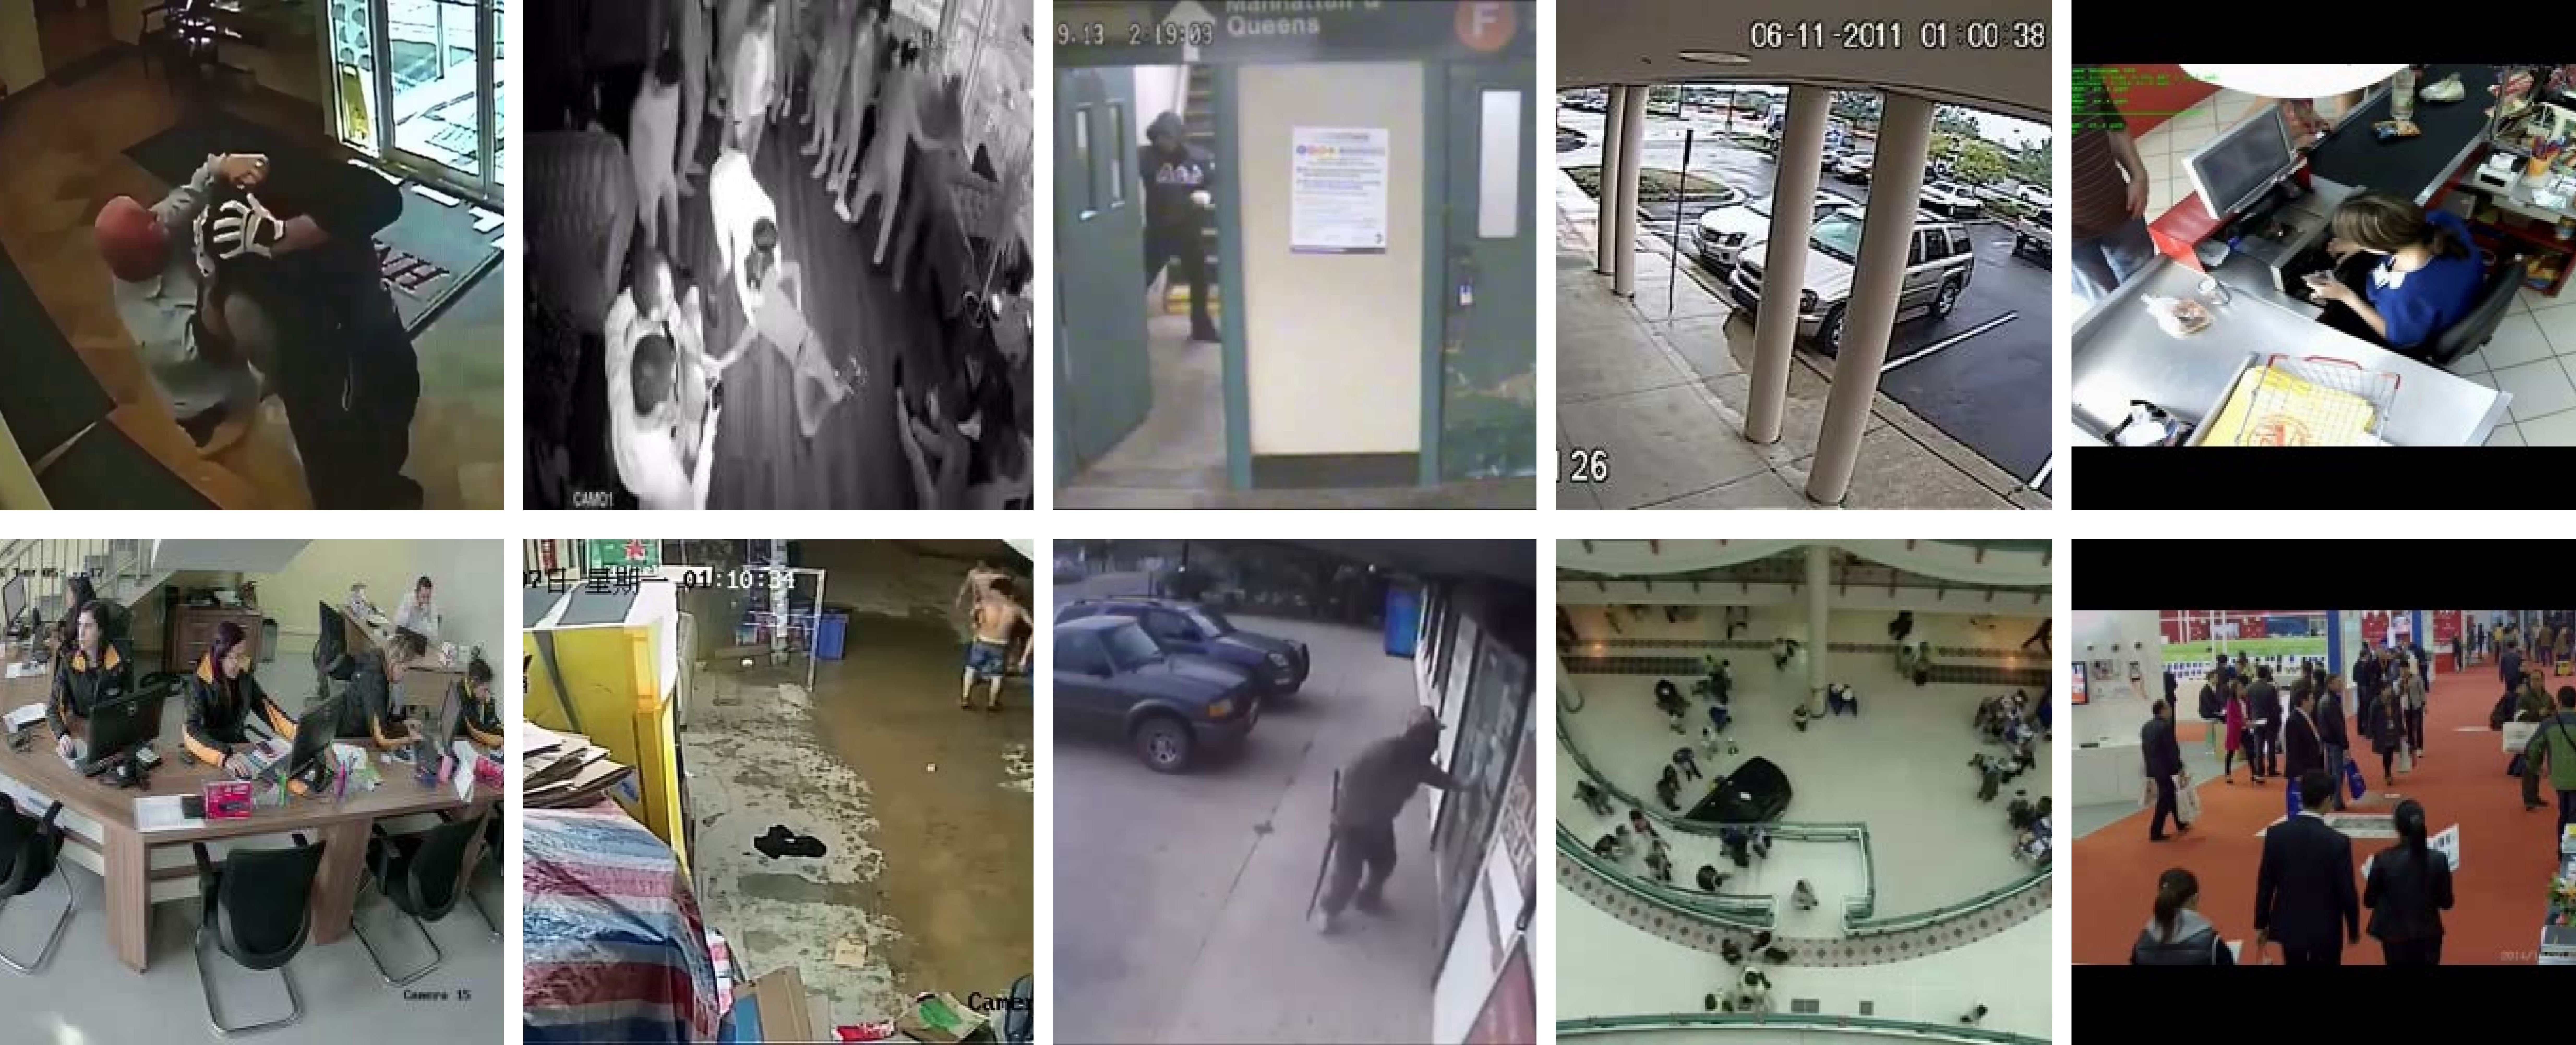
\includegraphics[width=0.9\linewidth]{Images/rwf_content.png}
        \caption{Contents of RWF-2000 Dataset}
        \label{rwf2000content}
    \end{figure}

%\clearpage
    
    % The RWF-2000 dataset stands out as a superior resource for violence detection research due to several key factors that are mentioned later. This dataset has emerged as the most suitable dataset for the intended purpose.\\

    \begin{figure}[h!]
        \centering
        \includegraphics[width=0.9\linewidth]{Images/RWF_Dataset.png}
        \caption{RWF-2000 Dataset Overview}
        \label{rwf2000overview}
    \end{figure}

% \clearpage

    Some of the advantages of RWF-2000 over other datasets for violence detection are in Table \ref{rwf2000adv} and Table \ref{rwf2000disadv}.
    
    % \begin{itemize}
    %     \item With over 2,000 video clips, the RWF-2000 dataset offers a substantial collection of data for training and evaluating violence detection algorithms. This large dataset size enables models to generalize well across diverse scenarios and contexts
    %     \item Each video clip in the RWF-2000 dataset is comprised of 150  frames (30fps  x 5 sec) making it of equal duration and similar size. This ensures that each video clip is balanced and the whole dataset has been limited to 2000x150 frames. 
    %     \item This dataset is also labeled with an equal split for both the classes containing 1000 clips each for the Fight and Non-Fight classes preventing class imbalances.
    %     \item The Dataset is arranged with a train-test split of 80\% training data (1600 samples) and 20\% testing data (400 samples), it is an ideal range for optimal performance results
    %     \item The RWF-2000 dataset is a widely used benchmark for violence detection research, serving as a standard reference point for evaluating the performance of different algorithms and technique
    % \end{itemize}

\vspace{1cm}

\begin{table}[h!]
\centering
\caption{Advantages of RWF-2000 Dataset}
\begin{tabular}{|c|p{12cm}|}
\hline
\textbf{No.} & \textbf{Feature}                                                                                                        \\ \hline
1            & The RWF-2000 dataset contains over 2,000 video clips, providing a substantial volume of data for training and evaluation. \\ \hline
2            & Each video clip consists of 150 frames (30fps x 5 sec), ensuring equal duration and size across the dataset.              \\ \hline
3            & The dataset is balanced with 1000 clips each for Fight and Non-Fight classes, avoiding class imbalances.                  \\ \hline
4            & Arranged with an 80\% train (1600 samples) and 20\% test (400 samples) split, ideal for optimal training and testing.     \\ \hline
5            & Widely recognized as a benchmark in violence detection research, it serves as a standard reference for algorithm evaluation. \\ \hline
\end{tabular}
\label{rwf2000adv}
\end{table}

\clearpage
\noindent The resolution distribution of the RWF-2000 dataset is given in Figure \ref{rwf2000resolutiondist}.    

\begin{figure}[h!]
\centering
    \includegraphics[width=0.8\linewidth]{Images/RWF-2000 Video Resolution freq bar plot.png}
    \caption{RWF-2000 Video Resolution Distribution}
    \label{rwf2000resolutiondist}
\end{figure}


% To address limitations such as low image quality, insufficient data quantity, videos with long durations but crude annotations, and hybrid sources merely resembling any realistic violence, RWF-2000  \cite{ourdataset}  emerged as the useful dataset for computer vision tasks. along with the Hockey Fight dataset which became important later on during the project development phase.
\end{enumerate}

\vspace{-5mm}

\begin{table}[h!]
\centering
\caption{Disadvantages of RWF-2000 Dataset}
\begin{tabular}{|c|p{12cm}|}
\hline
\textbf{No.} & \textbf{Disadvantage}                                                                                          \\ \hline
1            & Quality from YouTube varies widely, introducing inconsistencies that can affect model performance.              \\ \hline
2            & Use of specific keywords may miss some types of violence, leading to a biased dataset.                          \\ \hline
3            & Videos of real people used without consent raise ethical concerns and privacy issues.                           \\ \hline
4            & Models may overfit the types of violence in the dataset and won't generalize well.                             \\ \hline
5            & Lack of contextual information can make it difficult to distinguish between real and staged violence.           \\ \hline
6            & Potential legal issues related to copyright when using YouTube videos for research or commercial purposes.      \\ \hline
7            & Inaccuracies in video labeling can mislead training and affect detection system performance.                    \\ \hline
\end{tabular}
\label{rwf2000disadv}
\end{table}



% ----------------------------------------------------

\clearpage

\section{Dataset Preprocessing}

The Preprocessing begins with the transformation of raw video data, which undergoes initial preprocessing steps to enhance interpretability and facilitate downstream analysis. The data preprocessing encompasses the following steps:

\begin{itemize}
    \item Renaming the videos based on their content, such as labeling fight-related videos as "Fight\_1..." and "No\_Fight\_1...," for videos with no fight, which ensures better organization and understanding of the dataset. 

    \item Subsequently, the videos are subjected to frame extraction that decomposes the continuous video stream into individual frames. Each video's frames are then saved in a corresponding folder, named after the original video, simplifying data management and retrieval as shown in Figure \ref{processnormal}.
    

    \item Following frame extraction, the frames undergo resizing to a standardized format of 224x224 pixels with three color channels (224x224x3). This resizing ensures compatibility with most pre-trained deep learning models and facilitates efficient processing. While resizing maintains the essence of the video content, preserving three color channels balances the trade-off between training time, accuracy, and computational speed.

    \item Transforming data into the .npy format simplifies data management, data retrieval, and streamlining operations with efficient memory mapping. This optimization enhances read and write speeds, optimizing resource utilization for smoother training and inference processes.
\end{itemize}

    \noindent In the context of data handling, .npy files offer advantages over individual image files by consolidating multiple video frames into a single numpy array file. This simplifies the process of accessing and managing data, as users only need to interact with the .npy file instead of iterating through numerous image files placed inside different folders. The process of storing and searching in NumPy files is shown in Figure \ref{processnumpy}.\\

    \begin{figure}[h!]
        \centering
        \includegraphics[width=1\linewidth]{Images/without npy.png}
        \caption{Storing and Searching in Normal Files}
        \label{processnormal}
    \end{figure}

    \begin{figure}[h!]
        \centering
        \includegraphics[width=1\linewidth]{Images/With npy.png}
        \caption{Storing and Searching in NumPy Files}
        \label{processnumpy}
    \end{figure}

    \noindent Moreover, .npy files are stored in a binary format, resulting in smaller file sizes compared to collections of image files, which further enhances efficiency during data manipulation and storage. Figure \ref{memorymap} shows how the memory is mapped as a path to these .npy files.
    
    \begin{figure}[h!]
        \centering
        \includegraphics[width=0.9\linewidth]{Images/Mem map.png}
        \caption{Memory Mapping Printed as Path to the NumPy Files}
        \label{memorymap}
    \end{figure}

\noindent The combination of these preprocessing steps sets the stage for subsequent feature extraction and model training, enabling the development of a robust violence detection system. By transforming raw video data into a structured and standardized format, the project lays the foundation for effective analysis and interpretation. Additionally, the systematic organization of data enhances the scalability and reproducibility of the violence detection pipeline.

% ----------------------------------------------------

\clearpage

% \section{Model Building and Coding Practices}

% This section provides a detailed overview of the proposed system, outlining the technical procedures and methodologies used from initiation to completion, which includes descriptions of the model layers used, and the coding standards.

\section{Model Building}

% The proposed model was built to process videos sequentially, before the initial design of the model, the objectives were outlined clearly to make a model that is lightweight, fast, uses less computing, and is trainable in gaming laptops.

\begin{figure}[h!]
    \centering
    \includegraphics[width=0.9\linewidth]{Images/sys_high_level_overview.jpg}
    \caption{High-Level Overview of the Proposed System}\
    \label{fig:HighLevelOverview}
\end{figure}

\vspace{-5mm}

\noindent The design of the model started from a simple idea of \textit{how humans look and understand a violent situation}. Consider an example of a violent activity happening some distance away from a person, the person tends to focus on speech, disturbance, and movements. After some milliseconds the focus will be shifted to more detailed things in the view, like if a weapon is used, the emotional state of people surrounding the situation (anger, fear, and disgust) within a short duration of time the person will understand the situation and act accordingly. The team concentrated on building this type of response using deep learning methods, The initial focus of the person can be implemented using a special type of deep learning architecture called CNN which is an abstraction of human perception. To make the CNN focus on minute and detailed items present in the view the team used a simple attention mechanism called \textit{Spatial Attention}, which identifies the brightest(regions with high RGB values) and most averaged parts(repeated across many video frames, like quick movements) and makes a map out of it and compares with the original frames and returns the attended region which makes the important features stand out more during the network's learning process. But this Spatial Attention only helps to understand what is in a frame and where to focus. To act like a human, the network needs to know how the information changes over time, for this another deep learning architecture called LSTM was used. LSTMs are a type of 
Recurrent Neural Networks (RNN), that are designed to handle data in sequences. It has memory cells and other gates, which can maintain its state over time, effectively allowing the network to remember past information for an extended period. This is key to understanding temporal patterns and dependencies(time-based patterns).

\clearpage

\noindent Together CNN, Spatial Attention, and LSTM simulate the working of a human brain when the person is near a violent situation. But this can change with the situation (in technical terms, the data), as this biological response pattern is a general pattern for action recognition in humans, as for the proposed network architecture.


\noindent The high-level overview the proposed system consists of 6 different phases, each of which has a different deep learning architecture used. The diagrammatic representation of these phases can be seen in Figure \ref{fig:HighLevelOverview}. Details of each of these steps from data preprocessing to final output are described as follows.

% no clearpage here

\section{Detailed Description of the System}

\begin{figure}[!htbp]
    \centering
    \includegraphics[width=0.74\linewidth]{Images/prop_sys.jpg}
    \caption{Block Diagram of the Proposed System}\
    \label{fig:BlockDiagram}
\end{figure}

\noindent Figure \ref{fig:BlockDiagram} shows the architecture of the proposed system which is a simple but effective model construction that consists of different components working together to classify whether a video contains violence or not. The approach is a single-stream approach where the data sequentially goes through each layer of the model.

\clearpage

\subsection{Frame Extraction and Sampling: }

\noindent The preprocessing pipeline for video input begins with frame extraction, breaking down continuous streams into individual frames for subsequent analysis. Converting videos into sequential frames enables processing at the frame level, essential for analysis by computer vision models, facilitating action recognition and event detection in video data.

\noindent Resizing these frames to a standardized 224x224x3 format enhances computational efficiency and accelerates learning processes while reducing complexity. Standardizing resolutions ensures consistency across the dataset, enabling models to learn invariant features and improving generalization performance on unseen data. 

\noindent Converting frames into NumPy's .npy format optimizes storage and access, leveraging the format's efficient binary representation for faster read and write operations than traditional image file formats. Converting to .npy format streamlines data handling, reducing complexity and enabling efficient memory mapping for faster read and write operations, optimizing resource utilization during training and testing.

\noindent To maintain temporal context while managing computational resources effectively, a uniform sampling strategy is employed. This approach involves selecting frames at regular intervals, ensuring a balance between computational efficiency and the retention of essential information.

% \noindent Furthermore, the preprocessing pipeline sets the stage for subsequent feature extraction, where spatial and temporal features are extracted to capture relevant information from individual frames and temporal sequences. These features serve as inputs to downstream violence detection algorithms, contributing to improved accuracy and robustness in identifying violent activities within video streams. Thus, the preprocessing steps play a crucial role in optimizing computational efficiency, preserving temporal context, and enhancing the overall effectiveness of violence detection systems.

\subsection{Feature Extractor CNN}

\noindent The rich representations inside each frame of a video will be captured by feature extraction CNN models, in this case, the team has used a lightweight and fast pre-trained model named MobileNetV2, which is designed for the implementation on edge devices and provides a quick output. It is suggested in \cite{renjith_sir_paper} that effectiveness and accuracy can be improved by the usage of pre-trained models. 

\clearpage

\noindent The MobileNets uses a special kind of CNN called Depthwise Separable Convolution, it has a minor change from traditional CNN, as it splits the computation into two steps: depthwise convolution and pointwise convolution, the first applies a single convolution filter to each of the input channel and the later is used to create a linearly combined output of the depthwise convolution, these actions reduce the total number of multiplications required in computation than a traditional CNN. In the proposed model the 20 layers on the bottom of MobileNet were frozen, as there is no need to train the model to capture high-level details like edges, bright spots, etc.

\noindent But going to the top all other layers are trainable because it is required to capture minute details present in video frames. All of these operations are done using a special kind of layers called TimeDistributed layers, which do the corresponding operations to all the frames passed to the network in a batch. The code implementation is given below.

\begin{lstlisting}
from tensorflow.keras.applications import MobileNetV2
base_model = MobileNetV2(include_top=False, weights='imagenet', input_shape=input_shape[1:])
base_model.trainable = True
for layer in base_model.layers[:-20]: # Freeze last 20 layers
    layer.trainable = False
frames_features = TimeDistributed(base_model)(inputs)
\end{lstlisting}

\vspace{-5mm}

\subsection{Spatial Attention Mechanism :}

\noindent The output of MobileNetV2 is a group of feature maps that contains the spatial and temporal dimensions. The Spatial Features \cite{Spacial_feat} extracted from video frames capture static information, while temporal features \cite{Spacio-tempo} represent dynamic changes over time. The model needs special attention towards the spatial information, to focus on important parts of the frames, they are passed through a Spatial Attention module. This helps the model to improve its ability to capture important visual features associated with violence. The spatial attention works in a simple manner, where the maximum and average values across the frame batch are calculated and concatenated along the channel axis. 

\noindent This is then passed through a single filter CNN to make an activation map(shown in results and discussions) having values between 0 and 1. Finally, a multiplication operation is done against the feature map with the original input tensor element-wise, this multiplication operation basically acts as a gating mechanism where values close to 1 in the attention map allow the corresponding features in the input tensor to pass, and values close to 0 will be blocked. The code used for spatial attention is given below.

% \clearpage

\begin{lstlisting}
class SpatialAttention(Layer):
    def __init__(self, **kwargs):
        super(SpatialAttention, self).__init__(**kwargs)

    def build(self, input_shape):
        self.conv2d = Conv2D(1, (7, 7), activation='sigmoid', padding='same')
        super(SpatialAttention, self).build(input_shape)

    def call(self, inputs):
        max_pool = tf.reduce_max(inputs, axis=-1, keepdims=True)
        avg_pool = tf.reduce_mean(inputs, axis=-1, keepdims=True)
        concat = Concatenate(axis=-1)([max_pool, avg_pool])
        attention = self.conv2d(concat)
        return Multiply()([inputs, attention])
\end{lstlisting}


\subsection{Batch Normalization:}

\noindent Following the spatial attention mechanism and learning in general the distribution of activations in each layer may shift, leading to slower convergence and degraded performance. Batch normalization is a useful technique that can be applied to stabilize the activations, which helps improve the convergence and training speed of the model.

\subsection{Feature Pooling \& Concatenation:}

The output from batch normalization is then split into two branches. One branch is dedicated to GlobalAveragePooling2D, and the other to GlobalMaxPooling2D. These pooling operations reduce the size of feature maps and output combined information about the features. The results from both pooling operations are concatenated to capture comprehensive spatial information from the video frames.

\subsection{LSTM Network:}

\noindent The concatenated feature vector resulting from the pooling operations is then inputted into an LSTM network. LSTM networks are a type of RNN specifically designed for modeling sequential data and are proficient at capturing temporal dependencies and long-term patterns within sequences. In the context of video analysis, LSTM enables the model to effectively encode temporal information and identify complex patterns that extend over multiple frames. This is made possible by the presence of memory cells and gating mechanisms inside the LSTM. 

\subsection{Dense Layer \& Classification:}
Following the LSTM layer, the output(2D Tensor) is flattened using a Flatten layer(to 1D vector) and is passed through a collection of dense layer with dropout layers fitted between them to prevent overfitting. The final dense layer is followed by a softmax activation function to classify the output into two classes: violence or non-violence(labelled as 'Fight' and 'No Fight').

\noindent The key layers or components of the proposed system with its important functions are listed below in Table \ref{propsysfunc}. The summary of the model architecture is shown in Table \ref{table:modelsummary} while the model definition generated using the Keras Plotting utility is shown in Figure \ref{KerasBlockDiagram}.

\clearpage

\begin{table}[!htbp]
\centering
\caption[Key Components of Proposed System]{Key Layers/Components of Proposed System with Functions and Importance}
\begin{tabular}{|>{\raggedright\arraybackslash}m{4cm}|>{\raggedright\arraybackslash}m{5cm}|>{\raggedright\arraybackslash}m{5cm}|}
\hline
\textbf{Layer/Component} & \textbf{Function} & \textbf{Importance} \\ \hline
Frame Extraction & Converts video into sequential frames. & Essential for analyzing actions frame by frame. \\ \hline
Frame Resizing & Standardizes frame size to 224x224x3. & Ensures uniform input dimensions for consistent processing. \\ \hline
NumPy Conversion (.npy) & Optimizes frame storage and access. & Enhances data handling speeds and training efficiency. \\ \hline
Uniform Sampling & Selects frames at regular intervals. & Balances computational load and info retention. \\ \hline
Feature Extractor CNN (MobileNetV2) & Extracts features using depthwise separable convolutions. & Extract spatial features within frames. \\ \hline
Spatial Attention Mechanism & Highlights important spatial features in frames. & Focuses model on significant areas, improving detection accuracy. \\ \hline
Batch Normalization & Stabilizes activations, improve training efficiency. & Ensures faster, more stable training convergence. \\ \hline
Feature Pooling \& Concatenation & Reduces dimensionality and combines features. & Captures comprehensive spatial information from frames. \\ \hline
LSTM Network & Captures temporal dependencies and patterns across frames. & Essential for recognizing sequences of actions that indicate violence. \\ \hline
Dense Layer \& Classification & Processes features to classify the video as 'violence' or 'non-violence'. & Makes the final decision using learned features to detect violent behavior. \\ \hline
\end{tabular}
\label{propsysfunc}
\end{table}

\clearpage

\begin{figure}[htbp!]
    \centering
    \includegraphics[width=0.99\linewidth]{Images/our_model.jpg}
    \caption{Keras Plotting Utility's Output of Model Definition in Code}\
    \label{KerasBlockDiagram}
\end{figure}

\vspace{-10mm}

\begin{table}[H]
\centering
% \caption[Summary of Model Architecture]{Summary of Model Architecture(*TimeDistributed $|$ Total Parameters: 3,659,990)}
\caption{Summary of Model Architecture}
\begin{tabular}{c|c|c|c}
\hline
\textbf{Layer (type)}            & \textbf{Output Shape}       & \textbf{Param \#} & \textbf{Connected to}               \\ \hline
input\_1 (InputLayer)            & (None, 20, 224, 224, 3)     & 0                 & []                                   \\ 
MobileNetV2* & (None, 20, 7, 7, 1280)      & 2,257,984         & ['input\_1[0][0]']                   \\ 
Spatial Attention* & (None, 20, 7, 7, 1280)      & 99                & MobileNetV2*         \\ 
Batch Normalization* & (None, 20, 7, 7, 1280)      & 5,120             & Spatial Attention*      \\
GlobalAveragePooling2D* & (None, 20, 1280)            & 0                 & Batch Normalization*    \\
GlobalMaxPooling2D* & (None, 20, 1280)            & 0                 & Batch Normalization*     \\ 
Concatenate      & (None, 20, 2560)            & 0                 & GlobalAvg/MaxPooling2D*\\
lstm (LSTM)                      & (None, 128)                 & 1,376,768         & ['concatenate[0][0]']               \\ 
flatten (Flatten)                & (None, 128)                 & 0                 & ['lstm[0][0]']                      \\ 
dense (Dense)                    & (None, 128)                 & 16,512            & ['flatten[0][0]']                   \\ 
dropout (Dropout)                & (None, 128)                 & 0                 & ['dense[0][0]']                     \\ 
dense\_1 (Dense)                 & (None, 25)                  & 3,225             & ['dropout[0][0]']                   \\ 
dropout\_1 (Dropout)             & (None, 25)                  & 0                 & ['dense\_1[0][0]']                  \\ 
dense\_2 (Dense)                 & (None, 10)                  & 260               & ['dropout\_1[0][0]']                \\ 
dropout\_2 (Dropout)             & (None, 10)                  & 0                 & ['dense\_2[0][0]']                  \\ 
dense\_3 (Dense)                 & (None, 2)                   & 22                & ['dropout\_2[0][0]']                \\ \hline
\end{tabular}
\label{table:modelsummary}
\end{table}

\vspace{-12mm}

*TimeDistributed Layer $|$ Total Parameters: 3,659,990


\clearpage


\section{Coding Practices}

To make the model as per the objectives and ideas the team used top-of-the-line technologies available to make the proposed deep learning networks. And orchestrated the whole process of designing and testing the model using the industry-grade productivity software named Notion. Other tools used to make the model are outlined in the Table \ref{tab:programmingDetails}

\begin{table}[!htbp]
    \centering
     \caption{Programming and Deep Learning Framework Details}
    \begin{tabular}{|>{\raggedright\arraybackslash}p{4cm}|p{10cm}|}
        \hline
        \textbf{Item} & \textbf{Description} \\
        \hline
        Programming Language & Python\cite{python}, a programming language focused on readability and easiness of implementing ideas. \\
        \hline
        Python version & 3.10.11, the version that supports most libraries \\
        \hline
        Deep Learning Framework & TensorFlow 2.10\cite{tf_paper}, Keras 2.10\cite{keras} \\
        \hline
        Other Libraries & OS, Numpy, OpenCV, Pandas, Matplotlib, and Seaborn  \\
        \hline
        DL Architectures used & CNN, LSTM, GlobalAveragePooling2D, GlobalMaxPooling2D, Concatenation Layer, Flatten Layer, Dense Layer, and Dropout Layer. \\
        \hline
    \end{tabular}
    \label{tab:programmingDetails}
\end{table}

% version control - git

\begin{table}[!htbp]
\centering
\caption{Model Training Parameters}
\begin{tabular}{c|c}
\hline
\textbf{Parameter}             & \textbf{Value}                 \\ \hline
Mixed precision                & ON, float32                    \\ 
Batch Size                     & 4                              \\ 
Num\_Frames                    & 20                             \\ 
Height x Width of each frame   & 224 x 224                      \\ 
Num\_Channels                  & 3 (RGB)                        \\ 
Num\_Classes                   & 2 (Fight, No Fight)            \\
Learning Rate                  & 0.001 to 0.0009                \\ 
Loss Function                  & categorical\_crossentropy      \\ 
Optimizer                      & Adam                           \\
Output Activation              & Softmax                        \\
\end{tabular}
\label{tab:params}
\end{table}

\noindent The parameters were selected after a concise run with different arrangements of these parameters. Some other parameters were found to be working in certain types of problems in literature, like a thumb rule, when using categorical cross entropy as the loss function, put the num\_classes as 2 and output activation as Softmax, or else use num\_classes as 1, output activation as Sigmoid and the loss function should be binary cross entropy. The paper introduced by V Deepa Et. al \cite{DeepaMisPaper} suggest using Adam Optimizer with a learning rate of 0.01 for this type of classification problem to get an effective learning curve without much overfitting.

\noindent Since the project involves processing videos there is a requirement for high memory in Read Only Memory(ROM), Random Access Memory(RAM), and Graphics Processing Unit-Video Random Access Memory (GPU VRAM). During the training phase, the data has to be stored in RAM and when the training starts the data has to be moved to GPU memory. During the training, there will be another kind of memory usage like making intermediate tensors during backpropagation, and Frameworks like TensorFlow have their own memory overheads for managing computations.  But If the system memory or graphics memory is low, then the program will hit an Out-Of-Memory(OOM) Error, thereby halting the execution of the program.

\noindent To curb this problem, there are three methods the team has implemented: Frame Sampling, Adding Data Generators, and Setting Incremental Memory Growth for GPU.

\vspace{-5mm}

\begin{enumerate}

    \item Frame Sampling - Using a sampled set(uniform sampling, random sampling, cluster sampling) of frames rather than using all the frames of a video as the input to the model.

    \item Data Generators - Similar to generators in Python which yields the specified amount of data during execution. Data Generators are also used to make the required training data and input data augmentation on the fly, especially in tasks like video processing.

    \item Incremental GPU Memory Growth - Frameworks like TensorFlow do not have built-in automated memory usage limits, they tend to allocate arrays and tensors to the

\clearpage
    
    total available memory upfront to the execution. But there are options to specify the usage of memory incrementally, one of them is setting memory growth for GPUs in TensorFlow. This can be implemented in code by,
\end{enumerate}

% \clearpage

\begin{lstlisting}
gpus = tf.config.experimental.list_physical_devices('GPU')
if gpus:
    try:
        for gpu in gpus:
            tf.config.experimental.set_memory_growth(gpu, True)
    except RuntimeError as e:
        print(e)  # Memory growth must be set before GPUs have been initialized
\end{lstlisting}


\noindent $\bullet$ List of Callbacks: Perform specific actions at various stages of training. Some of the callbacks used in the code are shown below.

\begin{lstlisting}
checkpoint_cb = ModelCheckpoint(checkpoint_path, save_best_only=True, verbose=1)
reduce_lr_cb = ReduceLROnPlateau(monitor='val_loss', factor=0.2, patience=3, min_lr=0.001, verbose=1)
early_stopping_cb = EarlyStopping(monitor='val_loss', patience=20, verbose=1, restore_best_weights=True)
csv_logger = CSVLogger(os.path.join(res_path, "training_log.csv"), append=True)
\end{lstlisting}

\begin{figure}[!htbp]
    \centering
    \includegraphics[width=0.6\linewidth]{Images/training_log.png}
    \caption{Snapshot of Training Log}\
    \label{fig:TrainingLog}
\end{figure}

\clearpage

\begin{itemize}
    \item ModelCheckpoint: helps to keep checkpoints at a specific training point which helps to recover that point if subsequent training gets halted by some unforeseen circumstances. This is useful when training a large model or when there is a need to add more information to an existing model.

    \item ReduceLROnPlateau: Changes the learning rate when the specified metric (here, validation loss) is not improving. Learning Rate changes at the end of the previous epoch

    \item EarlyStopping: Used to stop training when the specified metric (here, validation loss) goes out of range (means, the training curve and validation curve go away from each other)

    \item CSVLogger: Stores a piece of training information like epoch count, training accuracy, testing accuracy, training loss, and validation loss onto a CSV file. Figure \ref{fig:TrainingLog} is a snapshot of CSVLogger which shows how the results are arranged in the Comma Separated File (CSV) file.    
\end{itemize}




\noindent $\bullet$ Learning Rate Scheduler: Keeps specified initial learning rate for the first five epochs (in this case) and then it will make changes to the learning rate. Learning Rate is changed at the beginning of the current epoch.

\begin{lstlisting}
def scheduler(epoch, lr):
    if epoch < 5:
        return lr
    else:
        return lr * tf.math.exp(-0.1)
lr_scheduler = LearningRateScheduler(scheduler)
\end{lstlisting}

% \lfoot{\textit{Departmant of Artificial Intelligence and Data Science, SJCET Palai}}
% \renewcommand{\footrulewidth}{0.4pt}
\chapter{Results and Discussions}
%%%%%%%%%%%%%%%%%%%%%%%%%%%%%%%%%%%%%%%%%%%%%%%%%%%%%%%%%%%%
%%%%%%%%%%%%%%%%%%%%  NEW SECTION   %%%%%%%%%%%%%%%%%%%%%%%%
%%%%%%%%%%%%%%%%%%%%%%%%%%%%%%%%%%%%%%%%%%%%%%%%%%%%%%%%%%%%
\setcounter{equation}{0}

\nomenclature{CAST}{Concatenation of Attention enhanced Spatial and Temporal features}
\nomenclature{TP}{True Positive}
\nomenclature{FP}{False Positive}
\nomenclature{TN}{True Negative}
\nomenclature{FN}{False Negative}
\nomenclature{XAI}{Explainable AI}

\section{Model's Prediction on Unseen Data}

\noindent The Figure \ref{fig:FightPred} and Figure \ref{fig:noFightPred} show the predictive power of the model when given by a .npy file as input, during this testing phase the layers like Batch Normalization and Dropout Layers will be off. The output(prediction) of the model will be an average of calculations of the input frames in the model, as the model goes on to attend all the frames to make a representation of the input file. 

\begin{figure}[htbp]
    \centering
    \includegraphics[width=1\textwidth]{Images/single_video_fight_pred.png}
    \caption{Model Prediction on a 'Fight' Video}
    \label{fig:FightPred}
\end{figure}

\begin{figure}[htbp]
    \centering
    \includegraphics[width=1\textwidth]{Images/single_video_no_fight_pred.png}
    \caption{Model Prediction on a 'No-Fight' Video}
    \label{fig:noFightPred}
\end{figure}


\section{Performance Evaluation}

In this section, the performance of the proposed model is checked using various metrics to assess its effectiveness and reliability in achieving the intended outcomes. The primary objective of the project was to propose a lightweight system, that does not overfit on the data and trains in reasonable hardware resources. Though with the training most of these objectives were covered, there is a need to analyze the model in-depth to understand whether the model is robust, fast, and effective to unseen data.

\begin{itemize}
    \item Dataset Used: Hockey Fight Dataset

    \item Evaluation Metrics: Accuracy, Precision, Recall, and F1 Score.

    \item Testing methodology: The model will be tested on a separate part of the dataset called the testing set, which consists of 200 Videos under the labels Fight and No\_Fight.
\end{itemize}

% \begin{table}[htbp!]
% \centering
% \captionof{table}{Training and Testing Metrics}
% \begin{tabular}{c|c|c|c}
% \hline
% \textbf{Criteria} & \textbf{Metric} & \multicolumn{2}{c}{\textbf{Value (\%)}} \\
% \cline{3-4}
%            &                  & \textbf{Training}    & \textbf{Testing} \\ \hline
% Graph     & Accuracy          & 95.00                & 92.00               \\
% Testing   & Accuracy          & 89.00                   & 89.00                \\
% \hline
% \end{tabular}

% \label{table:trainingTestingAccMetric}
% \end{table}

\clearpage

\subsection{Accuracy-Loss Graph}

The Accuracy-Loss Graph is an essential visual tool that illustrates the model's performance across its training and validation phases. Accuracy measures the proportion of true results (both true positives and true negatives) among the total number of cases the model has gone through. Loss, on the other hand, quantifies the error between the predicted values and the actual values, which shows the model's precision during training. Therefore, these graphs help in understanding the model's learning curve and pinpointing any overfitting or underfitting issues.

\begin{figure}[htbp]
    \centering
    \includegraphics[width=1\textwidth]{Images/acc graph.png}
    \caption{Accuracy versus Epoch Graph}
    \label{fig:AccGraph}
\end{figure}

\begin{figure}[htbp]
    \centering
    \includegraphics[width=1\textwidth]{Images/loss graph.png}
    \caption{Loss versus Epoch Graph}
    \label{fig:LossGraph}
\end{figure}

\begin{figure}[htbp]
    \centering
    \includegraphics[width=1\textwidth]{Images/acc_loss_vs_epoch.png}
    \caption{Accuracy and Loss versus Epoch in a Single Graph}
    \label{fig:AccLossGraph}
\end{figure}

\noindent From these Figures \ref{fig:AccGraph}, \ref{fig:LossGraph}, \ref{fig:AccLossGraph} it is clear that the model has shown good performance in training, as well as testing. The space between the accuracy curves shows whether the model is overfitting or not, but on keen observation, it is clear that there are no serious signs of overfitting. Also, the troughs and crests are due to the presence of noise and resolution problems of the videos in the dataset.

\clearpage

\subsection{Confusion Matrix}

The Confusion Matrix is a tabular representation of the classification power of the deep learning models. It encodes the values to find other metrics like Precision, Recall, and F1 Score. The confusion matrix of the proposed model is given in Figure \ref{fig:confMatrix}

\begin{figure}[!htbp]
    \centering \includegraphics[width=0.65\textwidth]{Images/conf_matrix.png}
    \caption{Confusion Matrix of the Proposed Model}
    \label{fig:confMatrix}
\end{figure}

\noindent Confusion Matrix Analysis:

\begin{enumerate}
    \item True Positive (TP): 96 (Top-left cell) - Correct predictions where the actual class is "Fight" and model predicted, "Fight".

    \item False Positive (FP): 18 (Bottom-left cell) - Times model incorrectly predicted "Fight" when the actual class was "No\_Fight".

    \item False Negative (FN): 4 (Top-right cell) - Times model incorrectly predicted "No\_Fight" when the actual class was "Fight".

    \item True Negative (TN): 82 (Bottom-right cell) - Correct predictions where the actual class is "No\_Fight" and the model also predicted "No\_Fight".
    
\end{enumerate}

\clearpage

\subsection{Accuracy}

\noindent Accuracy is a common performance metric in deep learning, particularly useful for classification problems. It measures the proportion of true results (both true positives and true negatives) to the total observations(true positives, false positives, true negatives, and false negatives). Accuracy is computed as in the general equation \ref{acc},

\begin{equation}
%\[
\text{Accuracy} = \frac{\text{Number of correct predictions}}{\text{Total number of predictions}} = \frac{TP + TN}{TP + TN + FP + FN}
\label{acc}
%\]
\end{equation}

\[
\text{Accuracy (Training/Testing)} = \frac{96 + 82}{96 + 82 + 4 + 18} = \frac{178}{200} = 89\%
\]

% The model shows good accuracy (89\%) and excellent precision for predicting "Fight" (96\%).
% - Recall for "Fight" is lower (84.2\%), indicating room for improvement in capturing all true "Fight" instances.
% - Low number of false positives (4) suggests the model is conservative in predicting "Fight".
% - Adjustments may be necessary based on specific performance goals, especially in terms of sensitivity (recall) for the "Fight" class.

\subsection{Precision}
In violence detection systems, precision is crucial because it measures how many of the detected instances of violence are actually correct. High precision means that when the system identifies an event as violent, there is a high probability that it truly is violent. With high precision, unnecessary panic or resource wastage is minimized. Precision is computed as in the general equation \ref{precision},

\begin{equation}
%\[
\text{Precision} = \frac{TP}{TP + FP}
\label{precision}
%\]
\end{equation}

\[
\text{Precision (Fight)} = \frac{96}{96 + 4} = \frac{96}{100} = 96\%
\]

\[
\text{Precision (No\_Fight)} = \frac{82}{82 + 18} = \frac{82}{100} = 82\%
\]

\subsection{Recall}
Recall is equally critical because it measures the system’s ability to detect all actual violent events captured in the video data. In the context of public safety and security, a high recall rate ensures that no violent incidents go undetected. This is particularly vital in surveillance systems used in public areas like schools, malls, or public transportation, where failing to detect an act of violence can have severe consequences. Recall is computed as in the general equation \ref{recall},

\begin{equation}
%\[
\text{Recall} = \frac{TP}{TP + FN}
\label{recall}
%\]
\end{equation}

\[
\text{Recall (Fight)} = \frac{96}{96 + 18} = \frac{96}{114} \approx 84.2\%
\]

\[
\text{Recall (No\_Fight)} = \frac{82}{82 + 4} = \frac{82}{86} \approx 95.3\%
\]

\subsection{F1 Score}

The F1 score becomes particularly important when balancing the trade-offs between precision and recall. In violence detection, it is often crucial to maintain a balance where both false positives (non-violent acts labeled as violent) and false negatives (violent acts not detected) are minimized. This balance is essential because both types of errors can have serious implications—false positives can lead to unnecessary interventions, while false negatives might allow violent situations to escalate. The F1 score provides a single metric that helps optimize the model during training and tuning to ensure an effective balance between identifying true violence and reporting non-violent activities. Precision is computed as in the general equation \ref{f1score},

\clearpage

\begin{equation}
%\[
F1 = 2 \cdot \frac{\text{Precision} \cdot \text{Recall}}{\text{Precision} + \text{Recall}}
\label{f1score}
%\]
\end{equation}

\[
F1 \text{(Fight)} = 2 \cdot \frac{0.96 \cdot 0.842}{0.96 + 0.842} \approx 89.7\%
\]

\[
F1 \text{ (No\_Fight)} = 2 \cdot \frac{0.82 \cdot 0.953}{0.82 + 0.953} \approx 0.882 \text{ or } 88.2\%
\]

\vspace{1.5cm}

% \begin{minipage}{0.5\textwidth}
% \centering
% \captionof{table}{Training and Testing Metrics}
% \begin{tabular}{c|c|c|c}
% \hline
% \textbf{Criteria} & \textbf{Metric} & \multicolumn{2}{c}{\textbf{Value (\%)}} \\
% \cline{3-4}
%            &                  & \textbf{Training}    & \textbf{Testing} \\ \hline
% Graph     & Accuracy          & 95.00                & 92.00               \\
% Testing   & Accuracy          & 89.00                   & 89.00                \\
% \hline
% \end{tabular}

% \label{table:trainingTestingAccMetric}
% \end{minipage}\hspace{0.03\textwidth}%
% \begin{minipage}{0.5\textwidth}
% \centering
% \captionof{table}{Fight vs No Fight Metrics}
% \begin{tabular}{c|c|c}
% \hline
% \textbf{Metric} & \multicolumn{2}{c}{\textbf{Value (\%)}} \\
% \cline{2-3}
%                 & \textbf{Fight}    & \textbf{No Fight} \\
% \hline
% Precision       & 89.00             & 82                \\
% Recall          & 89.00             & 95.3              \\
% F1-Score        & 88.95             & 88.2              \\
% \hline
% \end{tabular}

% \label{table:otherMetrics}
% \end{minipage}

\begin{table}[!htbp]
\centering
\captionof{table}{Training and Testing Metrics}
\begin{tabular}{c|c|c|c}
\hline
\textbf{Criteria} & \textbf{Metric} & \multicolumn{2}{c}{\textbf{Value (\%)}} \\
\cline{3-4}
           &                  & \textbf{Training}    & \textbf{Testing} \\ \hline
Graph     & Accuracy          & 95.00                & 92.00               \\
Testing   & Accuracy          & 89.00                   & 89.00                \\
\hline
\end{tabular}

\label{table:trainingTestingAccMetric}
\end{table}


\vspace{1.5cm}

\begin{table}[!htbp]
\centering
\captionof{table}{Fight vs No Fight Metrics}
\begin{tabular}{c|c|c}
\hline
\textbf{Metric} & \multicolumn{2}{c}{\textbf{Value (\%)}} \\
\cline{2-3}
                & \textbf{Fight}    & \textbf{No Fight} \\
\hline
Precision       & 96.00             & 82.00                \\
Recall          & 84.20             & 95.30              \\
F1-Score        & 89.70             & 88.20              \\
\hline
\end{tabular}

\label{table:otherMetrics}
\end{table}

\vspace{0.5cm}

\noindent In addition, the overall result values that were computed are written in Table \ref{table:trainingTestingAccMetric} and Table \ref{table:otherMetrics}. The accuracy metrics (given in Table \ref{table:trainingTestingAccMetric}) are different for graph and model testing, this is because of the usage of automatic mechanisms to save the best keras model file based on validation accuracy which is explained in the coding practices section.

\clearpage

\section{Spatial Attention Maps}

Spatial Attention Maps helps to highlight regions of interest within images or data, aiding in the interpretation and understanding of complex visual information. The original image acts as the input, and the spatial attention map overlays above the original image to produce an output as shown in Figure \ref{fig:attmap}.

\begin{figure}[h!]
\centering
\subfloat[Original Image] {\includegraphics[width=0.3\textwidth]
{Images/attn_maps/1.jpg}}
\hfill
\subfloat[Attention Map] {\includegraphics[width=0.3\textwidth]
{Images/attn_maps/output.png}}
\hfill
\subfloat[Resultant Attention Map] {\includegraphics[width=0.3\textwidth]
{Images/attn_maps/1.png}}
\caption{Steps in Generating Attention Map}
\label{fig:attmap}
\end{figure}

\begin{figure}[h!]
\centering
\subfloat[Original Image] {\includegraphics[width=0.45\textwidth]
{Images/attn_maps/2.jpg}}
\hfill
\subfloat[Attention Map] {\includegraphics[width=0.45\textwidth]
{Images/attn_maps/2.png}}
\caption{Correct Attention Map}
\label{fig:correctAttn}
\end{figure}

\begin{figure}[h!]
\centering
\subfloat[Original Image] {\includegraphics[width=0.45\textwidth]
{Images/attn_maps/4.jpg}}
\hfill
\subfloat[Attention Map] {\includegraphics[width=0.45\textwidth]
{Images/attn_maps/4.png}}
\caption{Wrong Attention Map 1}
\label{fig:wrongAttn1}
\end{figure}

\begin{figure}[h!]
\centering
\subfloat[Original Image] {\includegraphics[width=0.45\textwidth]
{Images/attn_maps/5.jpg}}
\hfill
\subfloat[Attention Map] {\includegraphics[width=0.45\textwidth]
{Images/attn_maps/5.png}}
\caption{Wrong Attention Map 2}
\label{fig:wrongAttn2}
\end{figure}

\clearpage

\begin{figure}[h!]
\centering
\subfloat[Original Image] {\includegraphics[width=0.325\textwidth]
{Images/attn_maps/7.jpg}}
\hfill
\subfloat[Learning Attention(A)] {\includegraphics[width=0.325\textwidth]
{Images/attn_maps/7_2.png}}
\hfill
\subfloat[Learning Attention(B)] {\includegraphics[width=0.325\textwidth]
{Images/attn_maps/7_1.png}}
\caption{Learning Happening in Attention}
\label{fig:learningAttn}
\end{figure}

\begin{itemize}
    \item Purpose: Spatial Attention Maps are used to visually highlight areas within an image that a computational model focuses on when making decisions or predictions. This can help researchers and engineers understand what parts of an image are marked important by the model.

    \item Process: The generated attention map is overlaid on the original images. These maps are color-coded or heat-mapped layers as shown in Figure \ref{fig:attmap}(b) that indicate the `attention` a model gives to different parts of an image when analyzing it. The correct attention map outputs are shown in Figure \ref{fig:correctAttn} and the wrong ones in the \ref{fig:wrongAttn1} and Figure \ref{fig:wrongAttn2}. In addition, Figure \ref{fig:learningAttn} shows how the learning takes place in attention maps over each iteration.

    \item Educational and Diagnostic Use: These attention maps cannot be used for improving the algorithms by tweaking them, but they serve an educational purpose. They can help explain to students and professionals how certain algorithms interpret visual data and what features the network prioritizes. This can be classified as a part of ExplainableAI (XAI)
    
\end{itemize}

\clearpage

\section{Discussions}

\noindent Training a deep learning model without any manual feature engineering to perform well on complex data like real-world fight and violence data is inherently a difficult procedure. In order to make it possible, one way is to make a very deep network with complex architecture that can absorb all the intricacies and nuances in the training data, another way is to do manual feature engineering like annotating the dataset to tell the model where the violence or fight is occurring. Both of these require heavy manual work to make it possible.

\noindent Some of the reasons that fuel the difficulties are that the data were mostly captured from CCTV visuals which has many problems like low resolution, distant and different camera angles views. To make a well-performing and lightweight model(as per the objective) we have to input a lot of data, do validation, and incorporate many precautions to handle edge cases like overfitting, OOM errors, and other problems that are explained in the proposed methodology chapter. But still, the model has managed to overcome these difficulties which were justified by the results of the testing.

\noindent Effectively, the performance metrics like the accuracy-loss graphs and confusion matrix, show insight into the effectiveness and efficiency of our model. Precision shows a measure of the model's exactness by indicating the proportion of positive identifications that were actually correct. Recall provides insight into the model's completeness, reflecting its ability to identify all relevant instances in the dataset. Finally, the F1 Score combines precision and recall into a single metric that captures both the false positives and false negatives. It is particularly useful when the balance between precision and recall is important.

%\begin{figure}
    %\centering
   % \includegraphics[width=0.95\textwidth, height=0.60\textheight]{Activity.jpg.jpeg}
    %\caption{Activity diagram}
%\end{figure}

\lfoot{\textit{Departmant of Artificial Intelligence and Data Science, SJCET Palai}}
\renewcommand{\footrulewidth}{0.4pt}
\chapter{Conclusion}

\setcounter{equation}{0}
% \section{Conclusion}
\noindent In the domain of human activity detection, particularly in identifying instances of violence, combating overfitting presents a significant challenge, even with the utilization of large and deep layered models\cite{overfit}. This challenge primarily occurred due to the complex nature of the model itself and the extraction of irrelevant features during training. To address this issue, the project undertook the development of a network with a less complicated architecture compared to existing models.\\
\noindent By employing a simpler architecture, the proposed network can be effectively trained on systems with standard specifications, eliminating the necessity for high-end computing resources. Moreover, we integrated additional mechanisms such as spatial attention, global average pooling, and global max pooling to augment the model's capability to extract relevant features while reducing the risk of overfitting.\\
\noindent The accuracy of the proposed model aligns closely with existing systems, the noteworthy accomplishment lies in the significant reduction of overfitting. Furthermore, the model architecture was carefully designed to prioritize computational efficiency and resource utilization\cite{comp_efficiency}. This strategic approach enables seamless deployment on edge devices with limited processing power, such as surveillance cameras, facilitating precise classification between violent and non-violent activities.

\clearpage

\noindent Finally, the proposed approach has made substantial progress towards achieving the project's objectives of developing a lightweight, faster, and compact model capable of accurately distinguishing between violent and non-violent activities. Through a combination of simplified architecture, feature enhancement mechanisms, and a focus on computational efficiency, the proposed model represents a promising solution for real-world deployment in scenarios where resource constraints are a primary concern.
 
%\begin{figure}
    %\centering
    %\includegraphics[width=1\textwidth, height=0.50\textheight]{sq.png}
    %\caption{Sequence diagram}
%\end{figure}

\section{Future Scope}

The future of violence detection using AI holds significant promise and potential for advancements in several key areas:

\begin{itemize}

    \item \textbf{Audio-Visual Cues Integration:} By combining visual and auditory information, these systems can better understand violent incidents, improving accuracy and reliability. The model that detects child violence from voice variation is an example.\cite{child_violence}

    \item \textbf{Predictive Classification:} Implementing a method that can identify the likelihood of violence on a per-frame basis before the violence has occurred and caused any harm by localizing the regions of the frame or the violent people in view.\cite{SepConvLSTM}

    \item \textbf{Security and Law Enforcement Alert:} Violence detection systems can be integrated with emergency services, such as police dispatch centers or emergency call centers. When a violent incident is detected, the system can automatically generate an alert and relay relevant information to dispatchers.

    \item \textbf{Privacy-Preserving Solutions:} As privacy concerns continue to grow, there is a need for AI-driven violence detection solutions that respect individuals' privacy rights. Future research may explore privacy-preserving techniques, such as federated learning\cite{Federated_Learn} and differential privacy, to ensure sensitive data remains secure and confidential.

\clearpage

    \item \textbf{Detecting Violent Activities Involving Weapons:} Continuous evaluation of additional standard datasets should encompass a broader range of violent activities, including those involving weapons\cite{lstm&bilstm}, which present unique challenges for detection algorithms due to their concealment and potential variability in appearance.

     %\item \textbf{Contextual Understanding:} Future research may focus on enhancing the contextual understanding of violent behavior, taking into account factors such as environmental conditions, social dynamics, and situational context.

     \item \textbf{Spectral Imaging:} Spectral imaging\cite{spectral_image} offers a unique set of capabilities for violence detection such as usage of the IR spectrum, allowing for the identification of weapons, bloodstains, chemical residues during very low lighting conditions, complete darkness, or even through obstacles.

 
\end{itemize}

\section{Limitations}
While the project has made significant progress in addressing overfitting and improving computational efficiency for violence detection, there are several potential limitations to consider:
\begin{itemize}

      \item\textbf{Generalization:} Despite efforts to reduce overfitting, there may still be instances where the model fails to generalize well to unseen data or variations in real-world scenarios. This could lead to misclassifications or reduced accuracy in certain situations.
     
     \item\textbf{Resource Constraints:} While the model aims to be computationally efficient, it may still require a certain level of processing power and memory, which could be prohibitive for deployment on extremely resource-constrained edge devices.
    
     \item\textbf{Scope Limitation:} While your model excels in detecting physical violence, it may not be equipped to identify other forms of violence, such as weaponized violence
    
    \item\textbf{Environmental Factors:} Variations in lighting conditions, camera angles, and environmental clutter (e.g., crowded spaces, occlusions) may impact the model's performance, leading to decreased accuracy or increased false positives/negatives in violence detection. 
\end{itemize}

\newpage

%\begin{figure}[h]
%\centering
%\includegraphics[scale=0.5]{1s.png}
%\caption{Registration page.}

%\centering
%\includegraphics[scale=0.5]{2s.png}
%\caption{Profile and Settings.}
%\end{figure}
%\newpage
%\begin{figure}[h]
%\centering
%\includegraphics[scale=0.8]{3s.png}
%\caption{Dashboard.}

%\end{figure}

\lfoot{\textit{Departmant of Artificial Intelligence and Data Science, SJCET Palai}}
\renewcommand{\footrulewidth}{0.4pt}

\chapter{Project Activities and Outreach}
%%%%%%%%%%%%%%%%%%%%%%%%%%%%%%%%%%%%%%%%%%%%%%%%%%%%%%%%%%%%
%%%%%%%%%%%%%%%%%%%%  NEW SECTION   %%%%%%%%%%%%%%%%%%%%%%%%
%%%%%%%%%%%%%%%%%%%%%%%%%%%%%%%%%%%%%%%%%%%%%%%%%%%%%%%%%%%%
\setcounter{equation}{0}

%\nomenclature{ICAECT}{International Conference on Advances in Electrical, Computing, Communications and Sustainable Technologies}

\nomenclature{IEEE}{Institute of Electrical and Electronics Engineers}
\nomenclature{ICDICI}{International Conference on Data Intelligence and Cognitive Informatics}

\section{ICDICI-2024 Conference Submission}
The 5th International Conference on Data Intelligence and Cognitive Informatics (ICDCI 2024) invites global researchers, scholars, and industry professionals to explore the intersection of data intelligence and cognitive informatics. With a focus on understanding information processing systems, the conference aims to foster the development of advanced cognitive informatics technologies. The proof and reply email of the conference is shown in Figures \ref{fig:confSubmitted} and \ref{fig:confReply} respectively. 
\begin{itemize}

\item \textbf{Conference Name:} 5th International Conference on
Data Intelligence and Cognitive Informatics (ICDICI 2024)

\item \textbf{Publication:} Institute of Electrical and Electronics Engineers 
 (IEEE)

\item \textbf{Conference Dates:} 18\textsuperscript{th}-20\textsuperscript{th} November, 2024

\item \textbf{Date of Submission:} 2\textsuperscript{nd} May, 2024

\clearpage

\item \textbf{Acceptance Intimation:} 12\textsuperscript{th} September, 2024 

\item \textbf{Conference Website}: \textit{https://www.icdici.com/}

\item Notably this Conference was listed by the official conference searching site of the IEEE.

\item The selected paper immediately after the conference presentation will be submitted to IEEEXplore Digital Library.

\vspace{1cm}

\end{itemize}

\begin{figure}[h]
    \centering
    \includegraphics[width=0.8\linewidth]{Images/new_conf.png}
    \caption{Proof of Research Paper Submission to ICDICI2024 Conference}
    \label{fig:confSubmitted}
\end{figure}

\vspace{1cm}

\begin{figure}[h]
    \centering
    \includegraphics[width=0.8\linewidth]{Images/conf_reply.png}
    \caption{Reply - 'Paper Received' from ICDICI2024 Conference}
    \label{fig:confReply}
\end{figure}

\clearpage

\section{Carmel College Project Competition}

\begin{figure}[htbp!]
    \centering
    \includegraphics[width=0.85\linewidth]{Images/main_p_team_at_carmel_clg.jpg}
    \caption[Project Team members attending Project Competition]{Project Team Members Attending Project Competition at Carmel College of Engineering, Alappuzha held on 29\textsuperscript{th} April 2024. From left: Ajay T Shaju, Emil Saj Abraham, Vishnuprasad KG, and Justin Thomas Jo}
    \label{ccetComp}
\end{figure}

\vspace{1cm}

\noindent The team members participated in a project competition hosted at Carmel College of Engineering, Alappuzha Figure \ref{ccetComp}. The project presentation emphasized key features including the lightweight model, its scope, and notably the stampede incident at CUSAT served as the project's motivation, which seems to be easily understood by the judges of what the team has done. This experience provided an opportunity for all team members to showcase and exchange ideas with like-minded individuals, receiving valuable insights in return. Moreover, it enabled the team members to appreciate and learn from other projects presented at the competition.\\

% Further discussion about the details presented in Figure 6.1 can provide more insights.
%\ref{ccetComp}

% \begin{figure}[htbp!]
%     \centering
%     \includegraphics[width=0.7\linewidth]{Images/main_p_team_at_carmel_clg.jpg}
%     \caption[Project Team members attending Project Competition]{Project Team Members Attending Project Competition at Carmel College of Engineering, Alappuzha held on 29\textsuperscript{th} April 2024}
%     \label{ccetComp}
% \end{figure}

% \section{Indian Institute of Information Technology Kottayam}

% Participated in a workshop at IIIT-Kottayam, collaborating with professors who provided invaluable input for our violence mitigation project. Their keen interest in our concept led to enlightening exchanges of ideas and suggestions, enriching our understanding and fueling our project's development.

\lfoot{\textit{Departmant of Artificial Intelligence and Data Science, SJCET Palai}}
\renewcommand{\footrulewidth}{0.4pt}
\addcontentsline{toc}{chapter}{\numberline{}References}
\bibliographystyle{IEEEtran}
\bibliography{references}

\lfoot{\textit{Departmant of Artificial Intelligence and Data Science, SJCET Palai}}
\renewcommand{\footrulewidth}{0.4pt}
\include{8_Vision_Mission}

\end{document}